\chapter{Searching for an \textit{(un)stable equilibrium}:
Experiments in Training Generative Neural Networks Without Data}
\label{ch:unstable_eq}

\section{Introduction}

This chapter details the first successful attempt in my PhD research in finding a way of training a generative neural network in a data divergent (or data agnostic) way. 
This work was the first published and peer-reviewed approach for training generative neural networks without data.
The original experiments were published as a short paper at the NerIPS 2019 Workshop on Machine Learning for Creativity and Design, in Vancouver, Canada \citep{broad2019searching}. 
I also presented this work again at the Colors of AI workshop at the International Conference of Computational Creativity in Jönkoping in 2024.
Chapter \ref{ch:impact} details the reception of the series of artworks \textit{(un)stable equilibrium} that resulted from these experiments. 

In that initial paper I documented 6 experiments, each training run become the artworks \textit{(un)stable equilibrium 1:1} through to \textit{(un)stable equilibrium 1:6} (Figure \ref{fig:c3:original-experiments}). Unfortunately due to the passage of time, and multiple computer and disk-drive failures, I have lost the original logs and training samples from these initial training run samples. 
Therefore the rest of the results presented in this paper of experiments are re-runs of the original experiments (as faithfully as I could make them). The results are similiar, but not identical to the ones in the original paper, as it was not possible to perfectly replicate these original experiments without the same initial training parameters, hyperparameters and sampling schedule. \S \ref{c7:sec:unstable_eq} details the reception and artistic presentation of the original training runs in more detail. 

\begin{figure}[!htbp]
    \centering
    \subfloat[]{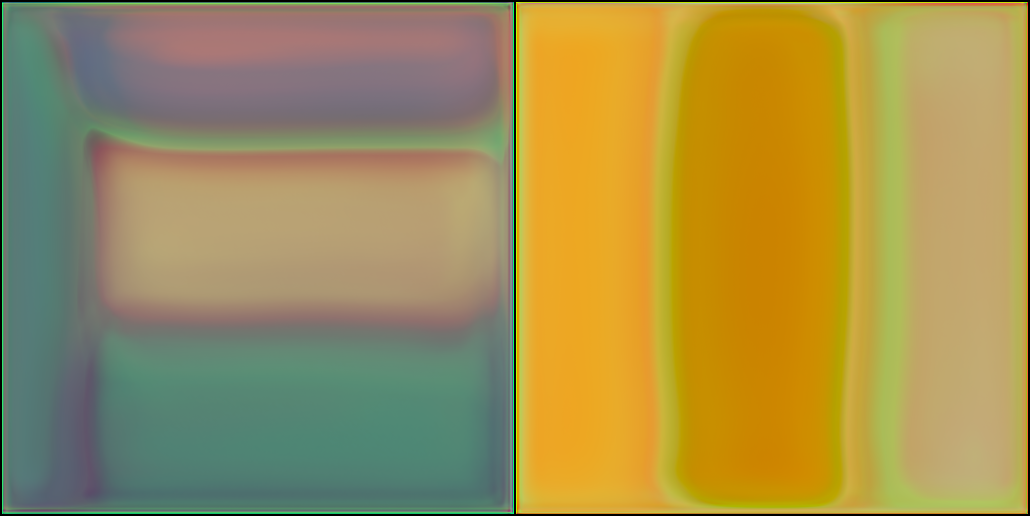
\includegraphics[width=0.45\textwidth]{figures/c4_unstable/original_experiments/1_1.png}}
    \hfill
    \subfloat[]{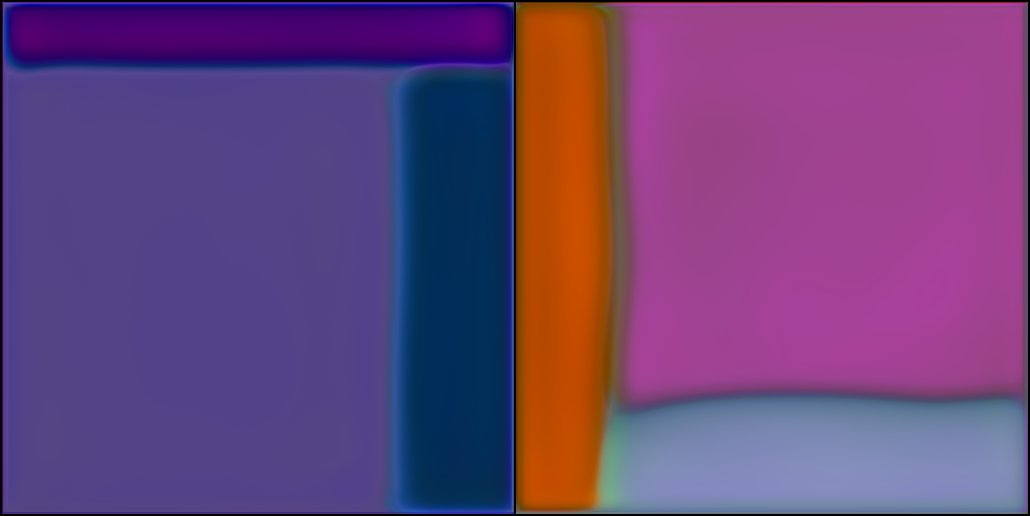
\includegraphics[width=0.45\textwidth]{figures/c4_unstable/original_experiments/1_2.png}}
    \hfill
    \subfloat[]{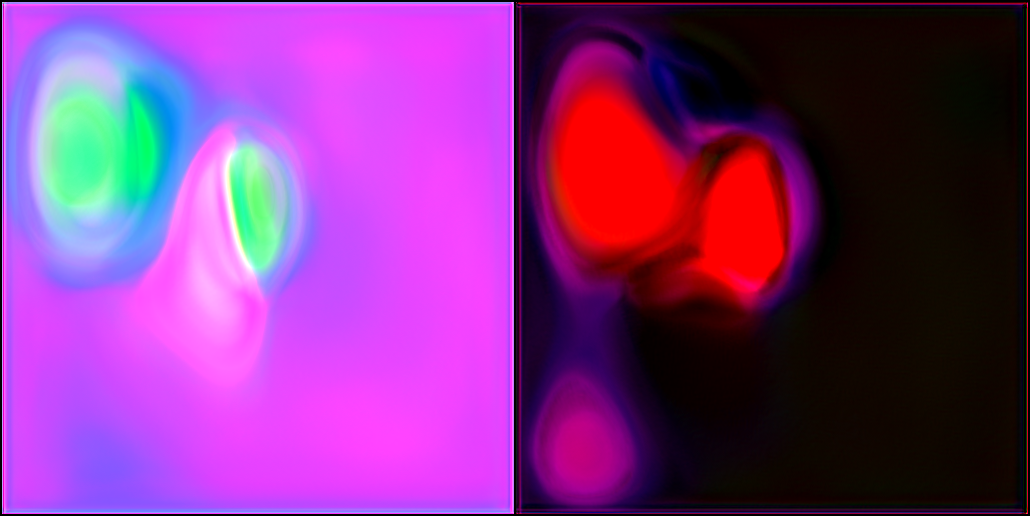
\includegraphics[width=0.45\textwidth]{figures/c4_unstable/original_experiments/1_3.png}}
    \hfill
    \subfloat[]{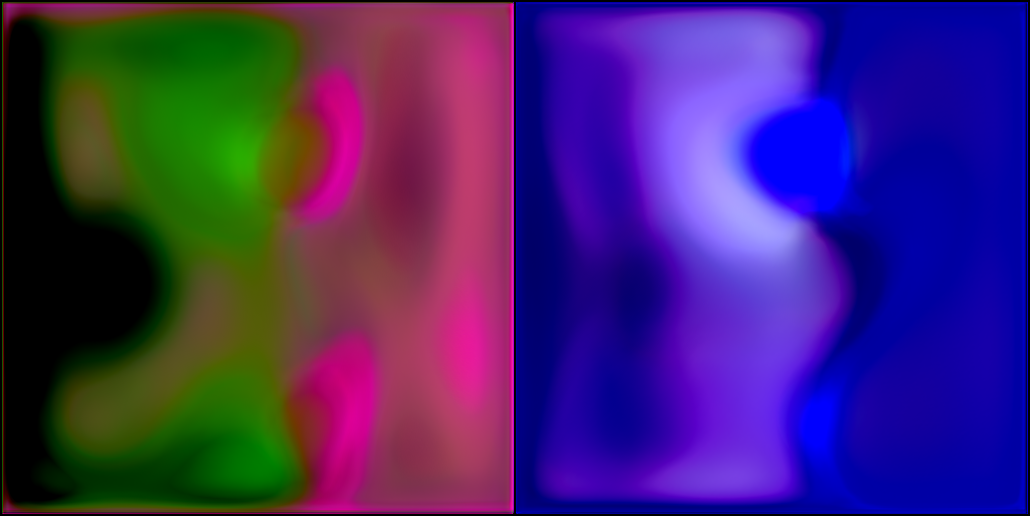
\includegraphics[width=0.45\textwidth]{figures/c4_unstable/original_experiments/1_4.png}}
    \hfill
    \subfloat[]{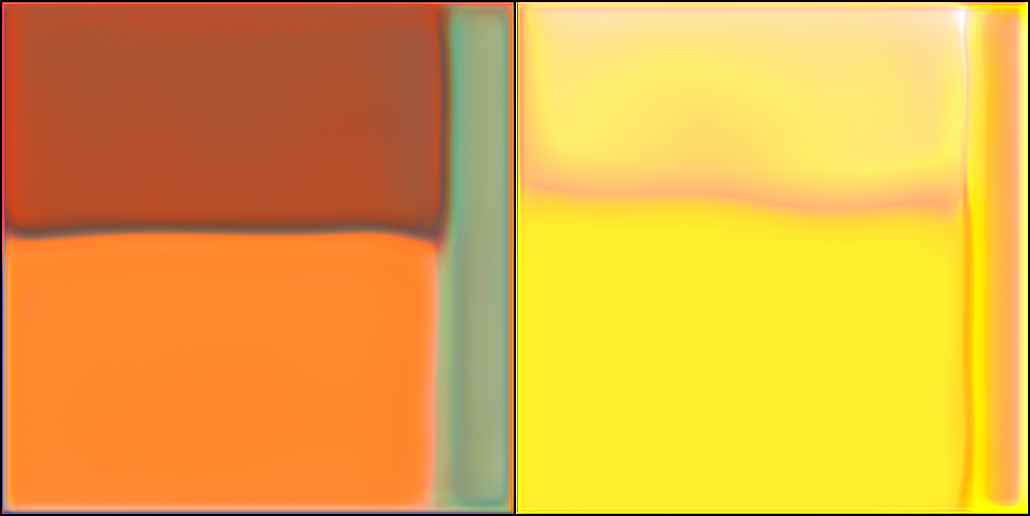
\includegraphics[width=0.45\textwidth]{figures/c4_unstable/original_experiments/1_5.png}}
    \hfill
    \subfloat[]{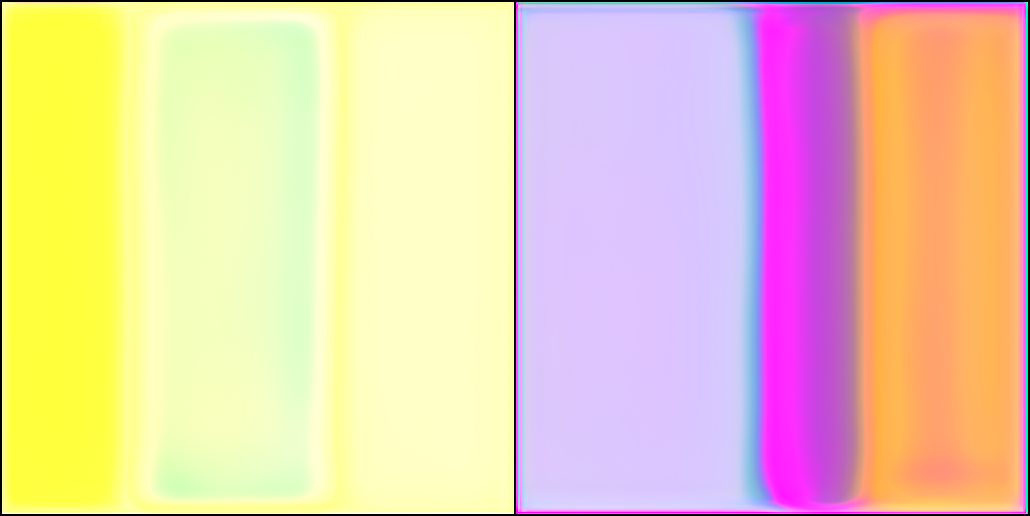
\includegraphics[width=0.45\textwidth]{figures/c4_unstable/original_experiments/1_6.png}}
    \caption[Original experiments in the \textit{(un)stable equilibrium} series]{Original experiments in the \textit{(un)stable equilibrium} series. (a) \textit{(un)stable equilibrium 1:1}, (b) \textit{(un)stable equilibrium 1:2}, (c) \textit{(un)stable equilibrium 1:3}, (d) \textit{(un)stable equilibrium 1:4}, (e) \textit{(un)stable equilibrium 1:5}, (f) \textit{(un)stable equilibrium 1:6}.}
    \label{fig:c3:original-experiments}
  \end{figure}

\section{Motivation}

This work came out of a deep frustration early on in my PhD journey, where I was trying to find ways of training generative models without modelling data.
It took me far longer than it should have to come to the realisation that this is an oxymoron. 
That a generative model is a model of a data distribution, and nothing more. 
Any attempt to move past this notion needed a completely different approach, and the first approach I developed which was fruitful is what is presented in this chapter. 

This work came out of a simple proposition: if it was possible to find a way of training a generative neural network without any training data, then by default, any outcome must be novel and could not resemble an existing training data distribution. 
There was little mathematical grounding to this approach. 
Through dogged trial and error, some playful reconfiguring of the most common (at the time) way of training generative models, GANs, I was able to find a way to train generative networks without data, in ways that produced at the very least, aesthetically interesting outcomes. 

This chapter tells the story of that process. 
Through the early experiments with configurations of models and loss functions that led to unremarkable results, through to the final configuration of models and training runs that resulted in the artworks \textit{(un)stable equilibrium}.
This chapter is named as such, because the journey I went on in producing those works was one of searching -- through intuition and aesthetic exploration -- for an (un)stable equilibrium. 
A balancing act of finding a system just chaotic enough to produce enough randomness in the resulting training run that enough unpredictable dynamics would lead to configuration of the weight parameters of the model such that unpredictable (and aesthetically compelling) results would come from the generator networks. 
But not enough for the loss functions to explode during training. 
The visual results of training were monitored, both visually by me as I inspected the generated output as each training increment progressed, along with a close monitoring of the fluctuations of the various loss functions throughout training. 
Over the course of a couple of intensive weeks of working in this unorthodox way, the configuration that produced these results was discovered. 

\section{Initial Experiments}

My first experiment took inspiration from the GAN framework (Figure \ref{subfig:c3:og-gan-diagram}) where a generator network imitates a training dataset, and the discriminator tries to tell them apart (Eq. \ref{eq:gan-loss}). 

\begin{equation} 
    Adv =\min_{G}\max_{D}\mathbb{E}_{x\sim p_{\text{data}}(x)}[\log{D(x)}])+  \mathbb{E}_{z\sim p_{\text{z}}(z)}[1 - \log{D(G(z))}]
    \label{eq:gan-loss}
\end{equation}

My initial adaptation of this was to replace the training data with another generator (Figure \ref{subfig:c3:double-gen-diagram}). 
In this arrangement the two discriminators are trying to imitate each other, whilst the discriminator is still trying to tell them apart (Eq. \ref{eq:double-gen-gan-loss}).

\begin{equation} 
    Adv = \min_{G_{1}}\max_{G_2}\max_{D}\mathbb{E}_{x\sim p_{\text{data}}(x)}[\log{D(x)}] +  \mathbb{E}_{z\sim p_{\text{z}}(z)}[1 - \log{D(G(z))}]
    \label{eq:double-gen-gan-loss}
\end{equation}

\begin{figure}[!htbp]
    \centering
    \subfloat[]{\label{subfig:c3:og-gan-diagram}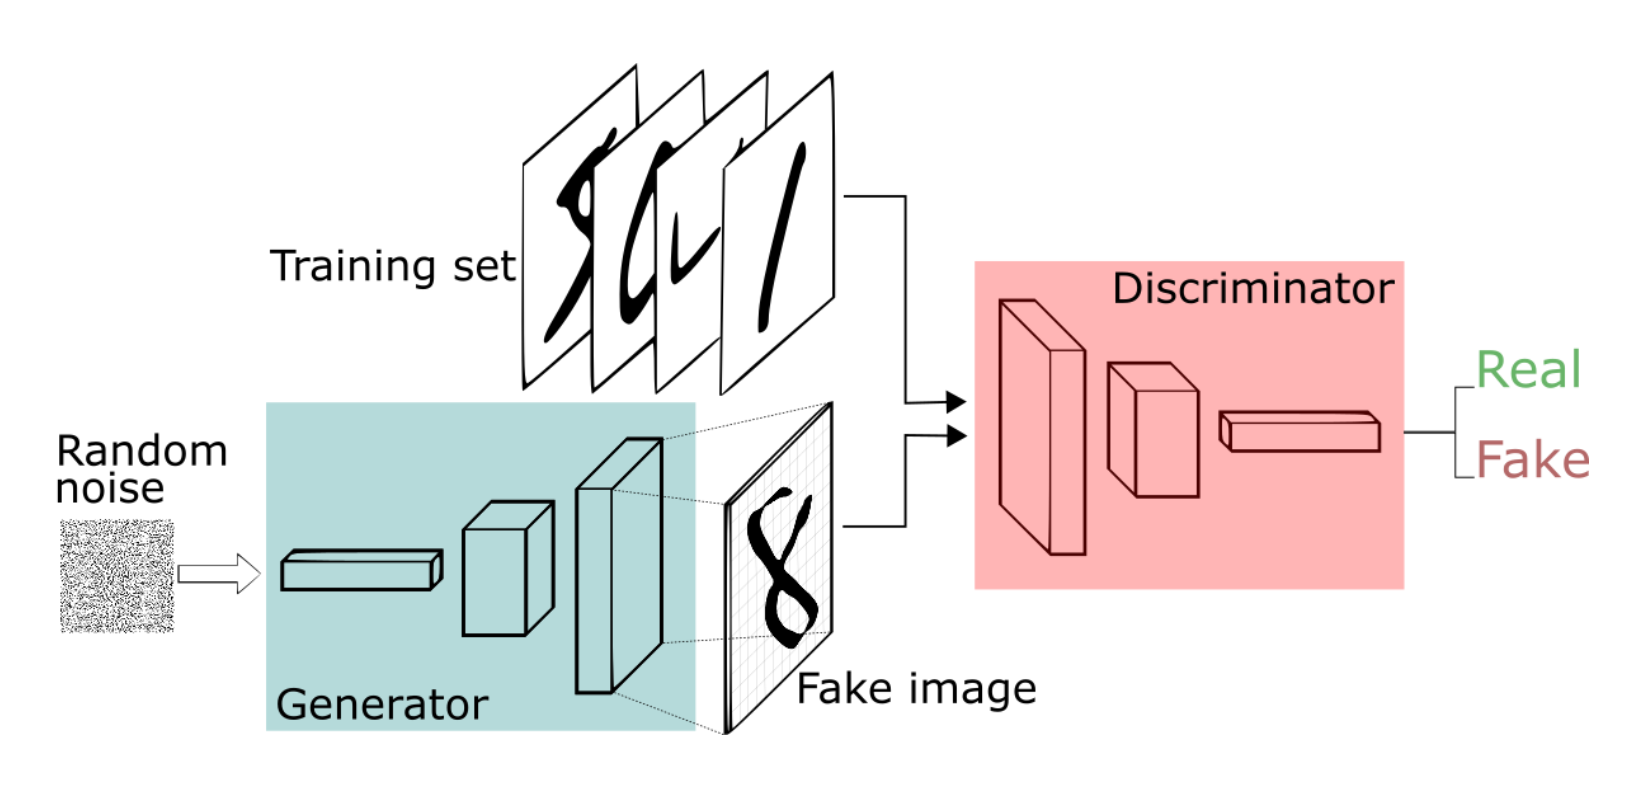
\includegraphics[width=0.75\textwidth]{figures/c4_unstable/diagrams/gan.png}}
    \hfill
    \subfloat[]{\label{subfig:c3:double-gen-diagram}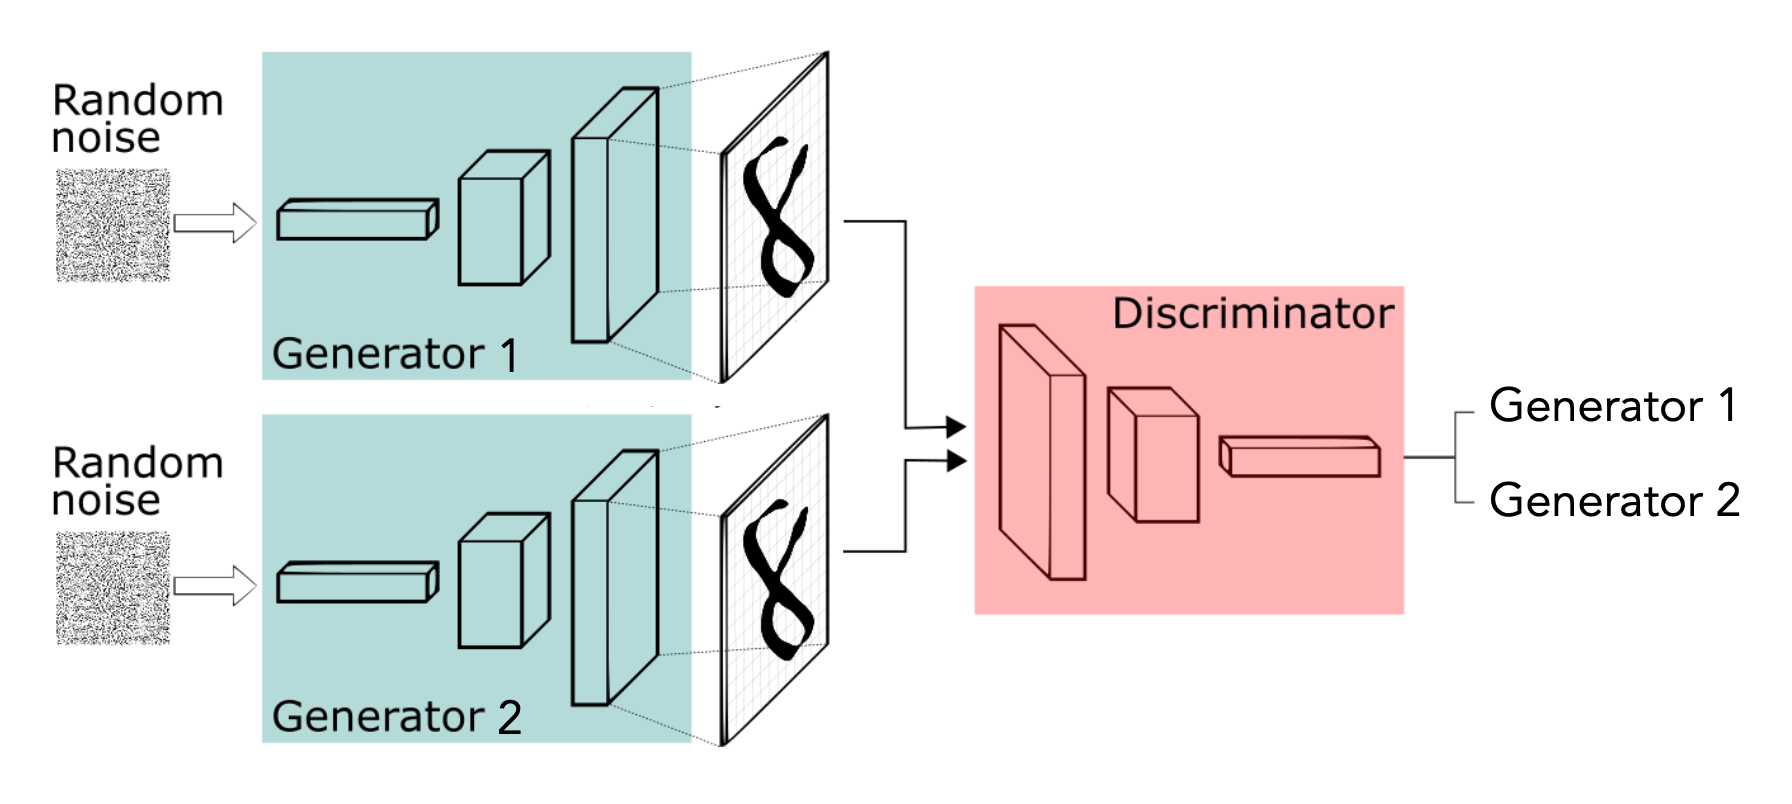
\includegraphics[width=0.75 \textwidth]{figures/c4_unstable/diagrams/two-generator.png}}
    \caption[GAN architecture training diagrams]{GAN architecture training diagrams. (a) The original GAN training framework where one generator imitates training data \citep{goodfellow2014generative}. (b) Novel training architecture where the training data is replaced with another generator in order to train two generative neural networks without data.}
    \label{fig:c3:gan-diagrams}
  \end{figure}

\subsection{Adversarial Loss}

Figures \ref{fig:c3:samples-no-col-var} \& \ref{fig:c3:no-var-losses} show the samples during training and loss logs during training respectively.
These experiments were done with the progressive growing GAN apprach \citep{karras2017progressive} that is used in the original StyleGAN \citep{karras2019style}, which is the model architecuture used in these training experiments.
The generator networks start training at a resolution of 32x32 pixels, and double in resolution for five steps, until reaching the final resolution of 512x512. 
Each generator is trained for 300 iterations at each resolution, totalling 1500 iterations for the full course of training.
In all of these experiments a fixed batch size of 10 was used for all resolutions in training (this was the largest I could perform at full resolution on a NVIDIA RTX 3090). 
The Adam optimiser was used for training \citep{kingma2014adam}, with a learning rate of $0.01$, and beta's $b_{1} = 0, b_{2} = 0.99$.

\label{c4:sec:og-loss}

\FloatBarrier
\begin{figure}[!htbp]
    \centering
    \subfloat[]{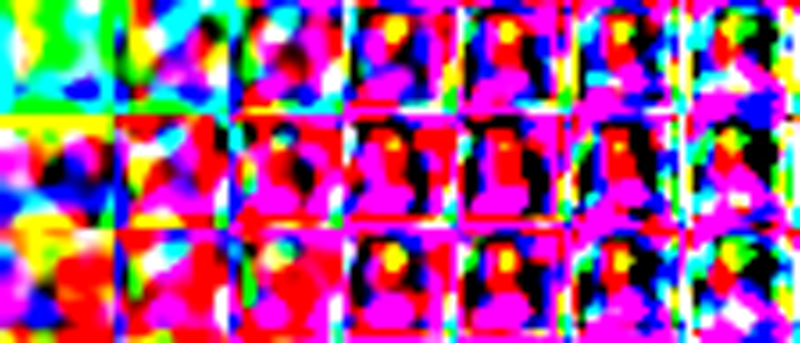
\includegraphics[width=0.45\textwidth]{figures/c4_unstable/train_samples/no_col_var/scaled_step_2_g1.png}}
    \hfill
    \subfloat[]{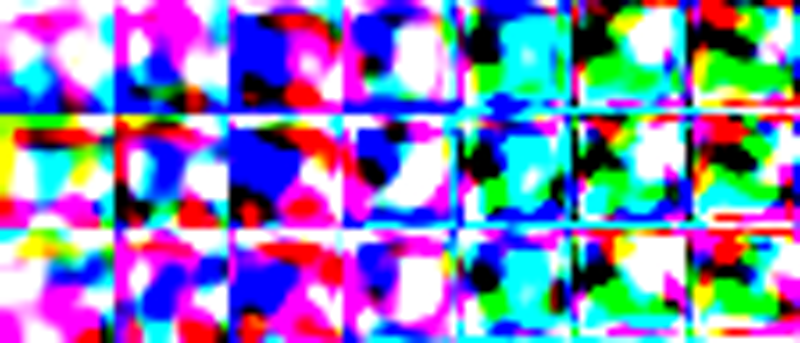
\includegraphics[width=0.45\textwidth]{figures/c4_unstable/train_samples/no_col_var/scaled_step_2_g2.png}}
    \hfill
    \subfloat[]{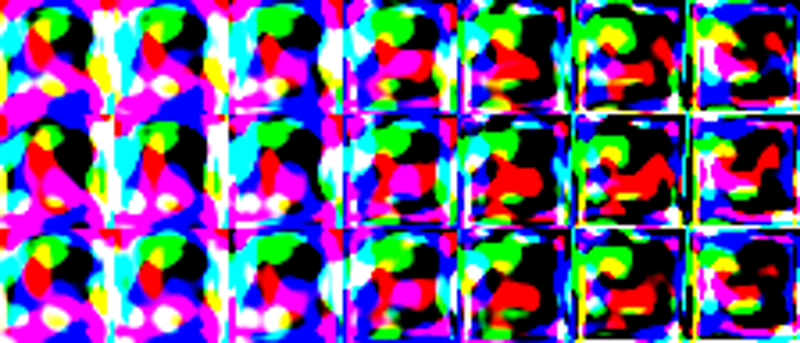
\includegraphics[width=0.45\textwidth]{figures/c4_unstable/train_samples/no_col_var/scaled_step_3_g1.png}}
    \hfill
    \subfloat[]{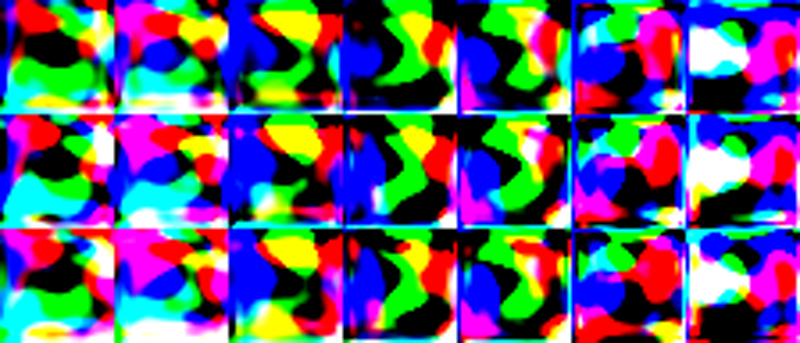
\includegraphics[width=0.45\textwidth]{figures/c4_unstable/train_samples/no_col_var/scaled_step_3_g2.png}}
    \hfill
    \subfloat[]{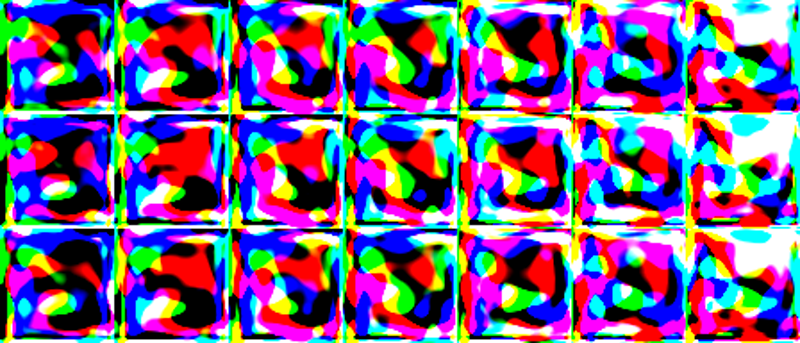
\includegraphics[width=0.45\textwidth]{figures/c4_unstable/train_samples/no_col_var/scaled_step_4_g1.png}}
    \hfill
    \subfloat[]{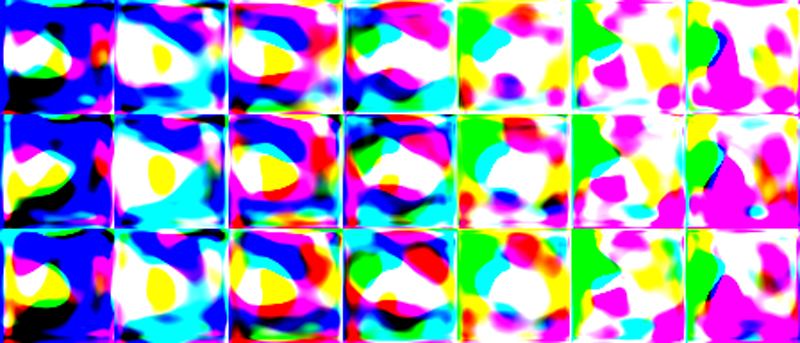
\includegraphics[width=0.45\textwidth]{figures/c4_unstable/train_samples/no_col_var/scaled_step_4_g2.png}}
    \hfill
    \subfloat[]{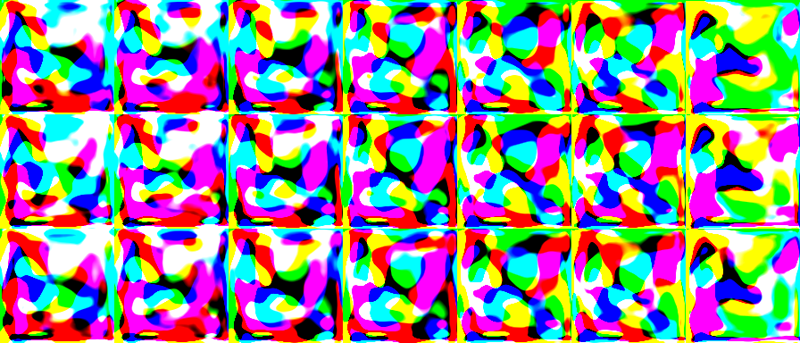
\includegraphics[width=0.45\textwidth]{figures/c4_unstable/train_samples/no_col_var/scaled_step_5_g1.png}}
    \hfill
    \subfloat[]{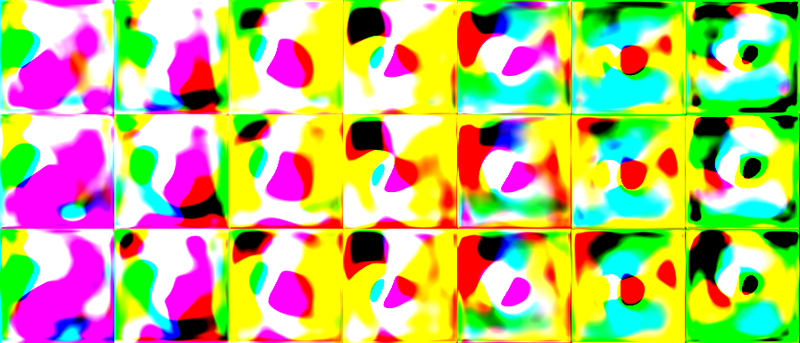
\includegraphics[width=0.45\textwidth]{figures/c4_unstable/train_samples/no_col_var/scaled_step_5_g2.png}}
    \hfill
    \subfloat[]{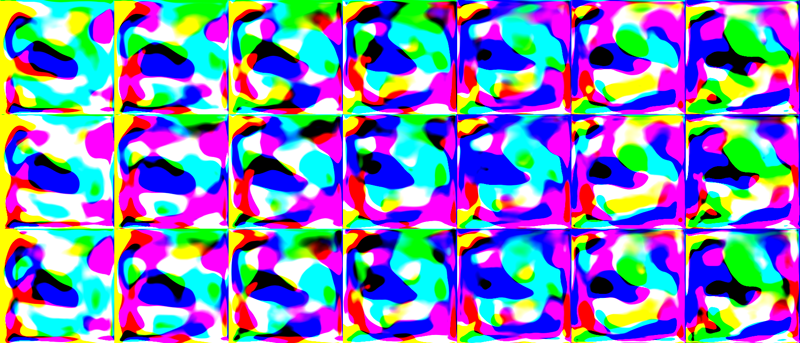
\includegraphics[width=0.45\textwidth]{figures/c4_unstable/train_samples/no_col_var/scaled_step_6_g1.png}}
    \hfill
    \subfloat[]{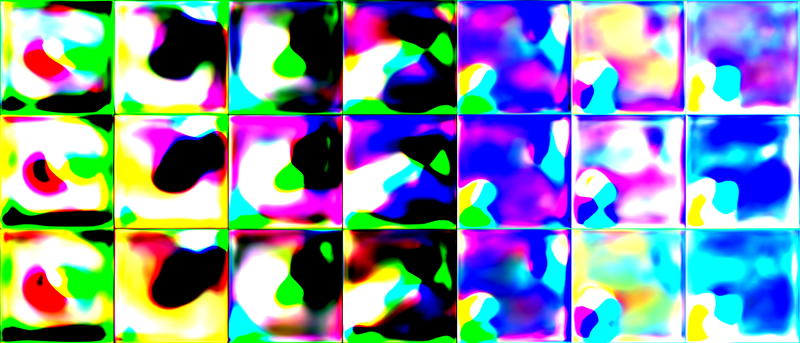
\includegraphics[width=0.45\textwidth]{figures/c4_unstable/train_samples/no_col_var/scaled_step_6_g2.png}}
    \hfill
    \caption[Training samples for standard adversarial training with two generators]{Training samples for standard adversarial training with two generators, sampled at increments of 50 iterations. The left column shows the training samples for $G_{1}$ and the right column shows the trianing samples for $G_{2}$. (a,b) Training samples at resolution 32x32 for iterations 0-300. (c,d) Training samples at resolution 64x64 for iterations 300-600. (e,f) Training samples at resolution of 128x128 for iterations 600-900. (g,h) Training samples at resolution 256x256 at iterations 900-1200. (i,j) Training samples at resolution 512x512 for iterations 1200-1500.}
    \label{fig:c3:samples-no-col-var}
  \end{figure}

  \begin{figure}[!htbp]
    \centering
    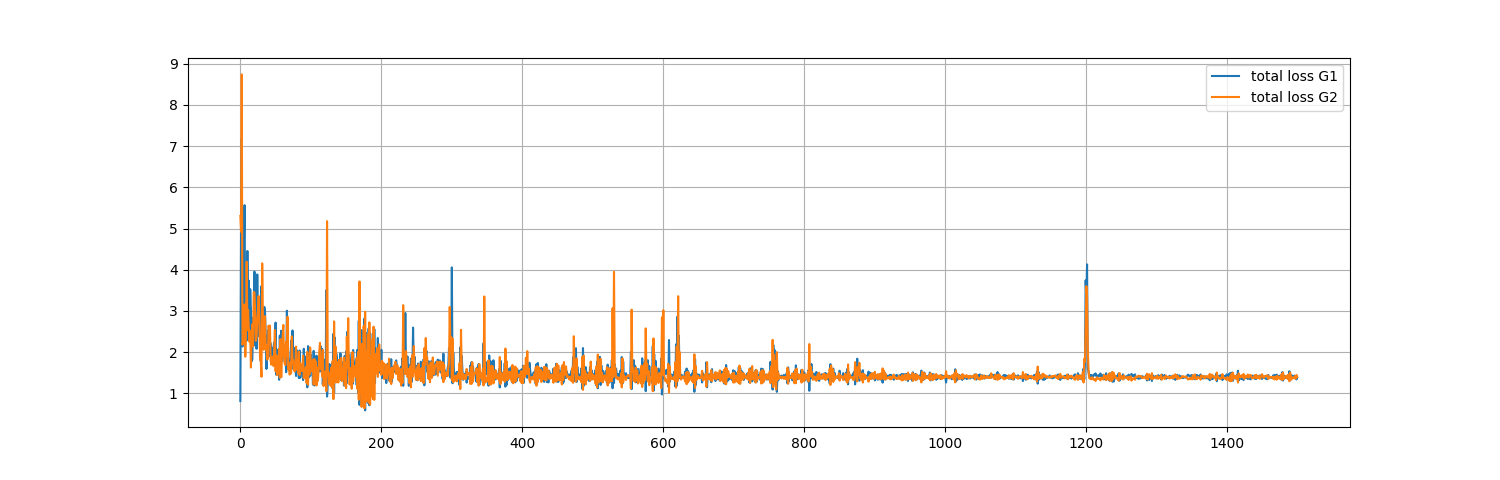
\includegraphics[width=1\textwidth]{figures/c4_unstable/train_losses/no_col_var/total_loss_no_var.png}
    \caption[Loss plot for double adversarial training]{Loss plot for double adversarial training of the two generator networks. Note: the loss for the discriminator is the same as the second generator.}
  \label{fig:c3:no-var-losses}
  \end{figure}

In this setting the visual results (Figure \ref{fig:c3:samples-no-col-var}) were not what I was hoping for.  
There is little diversity across the training batch for both generators. 
Essenitally, this training regime has suffered from mode collapse, which is a common failure state for GANs where the generator collapses into generating a single output in the output data distribution. 

In the normal GAN training regime, this diversity in the output images comes from mimicking the training data, which should have a wide variety of data samples in it (aka modes). 
Without training data, it is not surpirsing then that these models quickly collapse to a single mode of generation for each of the respective generators. 
To overcome this I needed to add an additional term to force to model into producing more diverse outputs. 
This is detailed in the following subsection.

\subsection{Colour Variance Loss Term}

In response to the mode collapse suffered in the previous experiment I developed an additional loss function to the training regime of this two generator training regime.
The additional loss term was designed to force increased colours to be used was to measure the batch-wide variance of values for each pixel, in each channel of the tensor. 
This term calculates the variance across the sampled batch $B$ for the respective channel c of the tensor for the samples drawn from both generators $g_{1}$ and $g_{2}$, which are then subtracted from each other (depending on which loss is being calculated for which generator) to enforce a relative variance that is higher than the other model across the different channels of the sample tensor.

\begin{equation}
    \label{eq:variance-gan}
    Vdiff = Var(B_{g_{1}}^{c}) - Var(B_{g_{2}}^{c})
    \end{equation}

This is calculated for the 4 channels of the tensor present in the sample batch. 
The first channel is the overall batch bt, the following channels are the colour channels of the output images: red r, green g and blue b.

\begin{equation}
    \label{eq:total-gan}
        Vdiff(B_{g_{1}}^{bt} , B_{g_{2}}^{bt}) + Vdiff(B_{g_{1}}^{r} , B_{g_{2}}^{r}) + Vdiff(B_{g_{1}}^{g} , B_{g_{2}}^{g}) +  dVdiff(B_{g_{1}}^{b} , B_{g_{2}}^{b}) 
    \end{equation}

The loss penalty was calculated for each generator with respect to the other. 
Therefore each generator was optimised to have more mini-batch variance than the other. 
Adding this term made a significant impact to the training. Eq. \ref{eq:gan-g1-col-var} shows the training objective for $G_{1}$ and Eq.  \ref{eq:gan-g2-col-var} shows the training objective for $G_{2}$.

\begin{equation} 
    G_{1}\ loss = \min_{G_{1}}Adv + Var(B_{g_{1}}^{c}) - Var(B_{g_{2}}^{c})
    \label{eq:gan-g1-col-var}
\end{equation}

\begin{equation} 
    G_{2}\ loss = \max_{G_{2}}Adv + Var(B_{g_{2}}^{c}) - Var(B_{g_{1}}^{c})
    \label{eq:gan-g2-col-var}
\end{equation}

Figures \ref{fig:c3:samples-col-var} \& \ref{fig:c3:col-var-losses} show the samples during training and loss logs during training respectively.

\begin{figure}[!htbp]
    \centering
    \subfloat[]{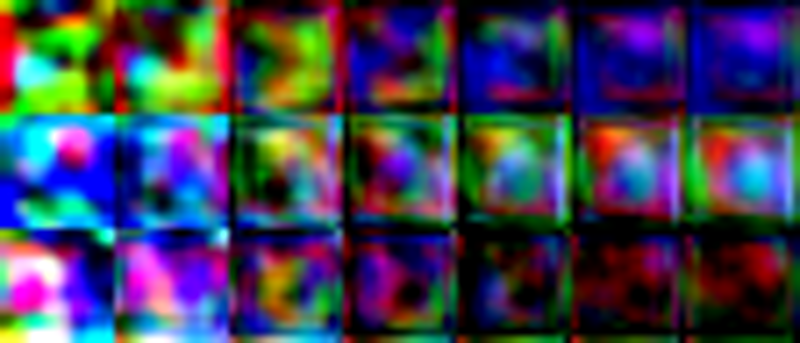
\includegraphics[width=0.45\textwidth]{figures/c4_unstable/train_samples/col_var/scaled_step_2_g1.png}}
    \hfill
    \subfloat[]{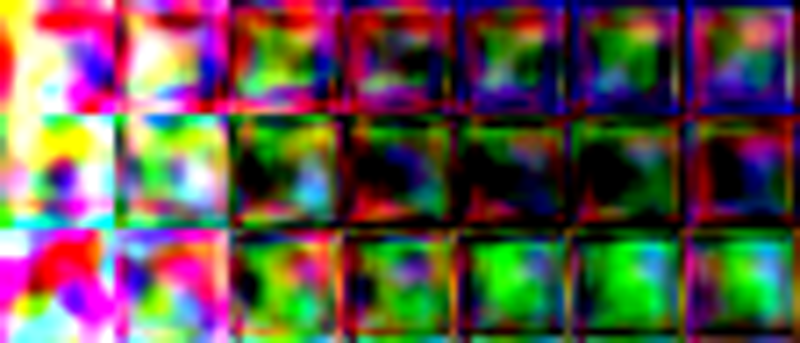
\includegraphics[width=0.45\textwidth]{figures/c4_unstable/train_samples/col_var/scaled_step_2_g2.png}}
    \hfill
    \subfloat[]{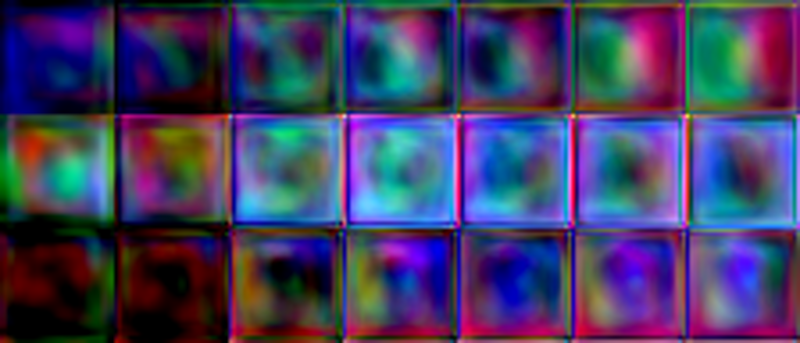
\includegraphics[width=0.45\textwidth]{figures/c4_unstable/train_samples/col_var/scaled_step_3_g1.png}}
    \hfill
    \subfloat[]{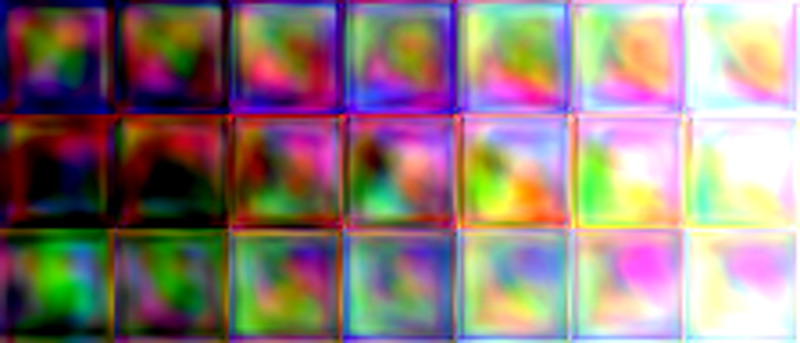
\includegraphics[width=0.45\textwidth]{figures/c4_unstable/train_samples/col_var/scaled_step_3_g2.png}}
    \hfill
    \subfloat[]{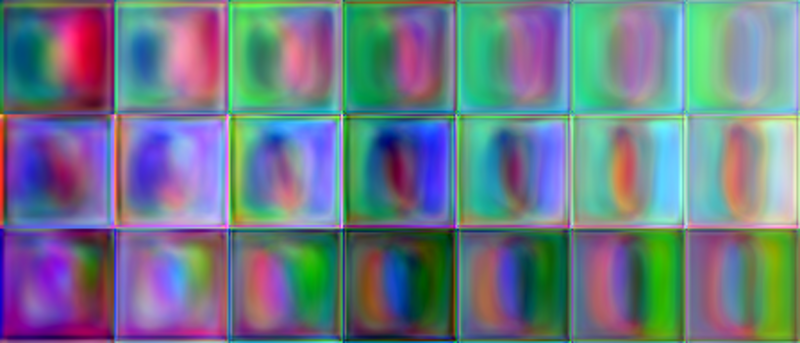
\includegraphics[width=0.45\textwidth]{figures/c4_unstable/train_samples/col_var/scaled_step_4_g1.png}}
    \hfill
    \subfloat[]{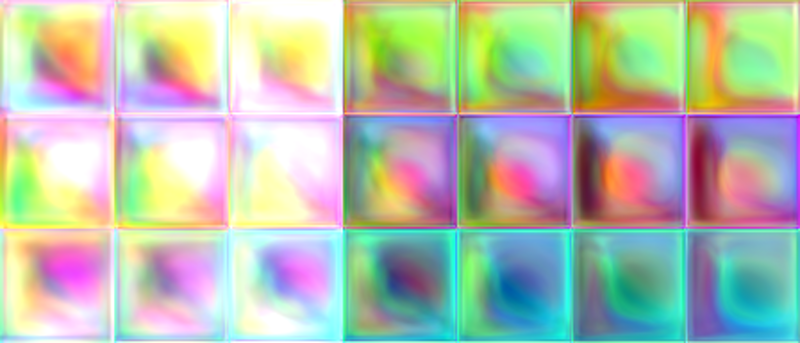
\includegraphics[width=0.45\textwidth]{figures/c4_unstable/train_samples/col_var/scaled_step_4_g2.png}}
    \hfill
    \subfloat[]{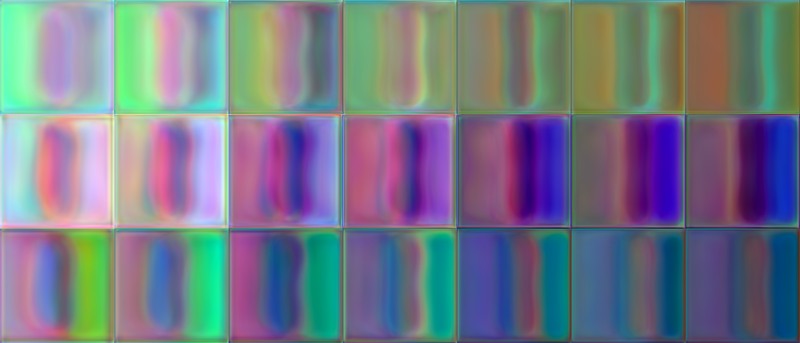
\includegraphics[width=0.45\textwidth]{figures/c4_unstable/train_samples/col_var/scaled_step_5_g1.png}}
    \hfill
    \subfloat[]{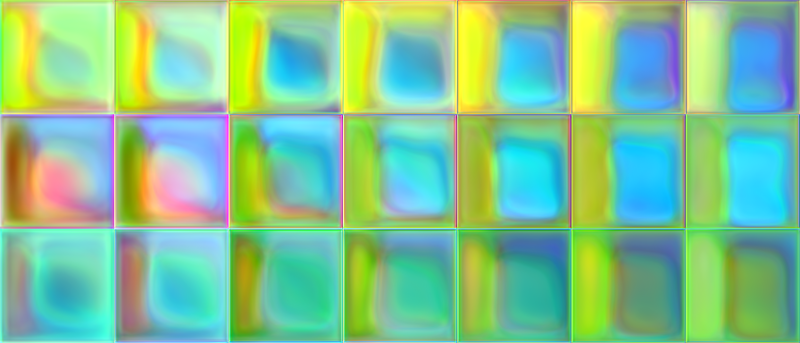
\includegraphics[width=0.45\textwidth]{figures/c4_unstable/train_samples/col_var/scaled_step_5_g2.png}}
    \hfill
    \subfloat[]{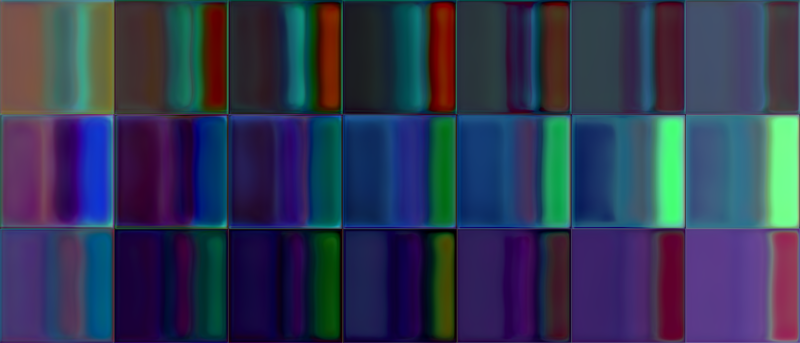
\includegraphics[width=0.45\textwidth]{figures/c4_unstable/train_samples/col_var/scaled_step_6_g1.png}}
    \hfill
    \subfloat[]{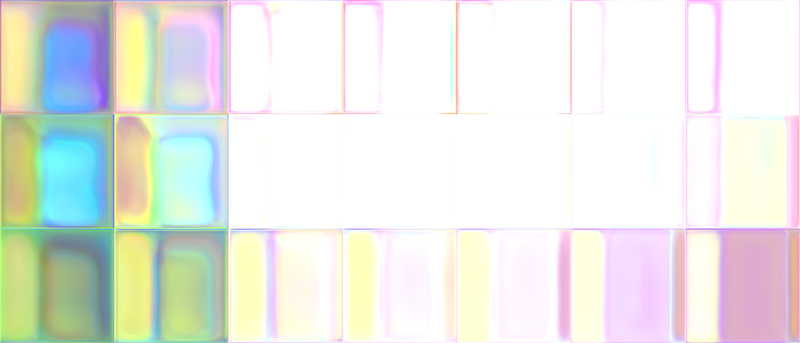
\includegraphics[width=0.45\textwidth]{figures/c4_unstable/train_samples/col_var/scaled_step_6_g2.png}}
    \hfill
    \caption[Training samples for adversarial training with two generators with the colour variance loss]{Training samples for adversarial training with two generators with the colour variance loss, sampled at increments of 50 iterations. The left column shows the training samples for $G_{1}$ and the right column shows the trianing samples for $G_{2}$. (a,b) Training samples at resolution 32x32 for iterations 0-300. (c,d) Training samples at resolution 64x64 for iterations 300-600. (e,f) Training samples at resolution of 128x128 for iterations 600-900. (g,h) Training samples at resolution 256x256 at iterations 900-1200. (i,j) Training samples at resolution 512x512 for iterations 1200-1500.}
    \label{fig:c3:samples-col-var}
  \end{figure}

  \begin{figure}[!htbp]
    \centering
    \subfloat[]{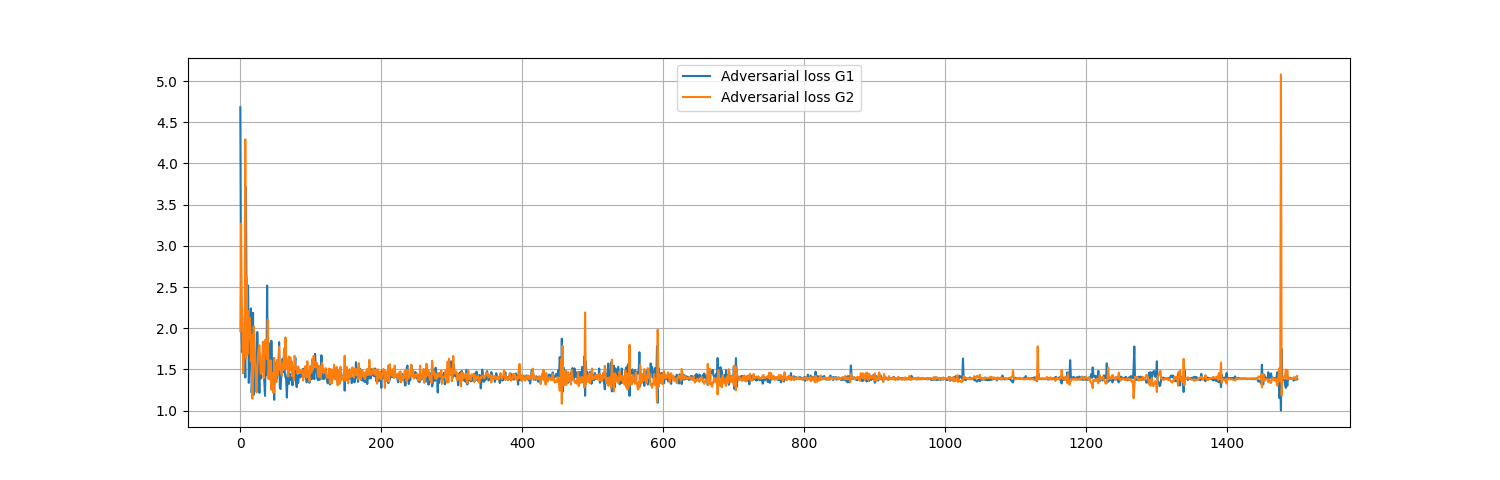
\includegraphics[width=1\textwidth]{figures/c4_unstable/train_losses/col_var/adversarial_loss.png}}
    \hfill
    \subfloat[]{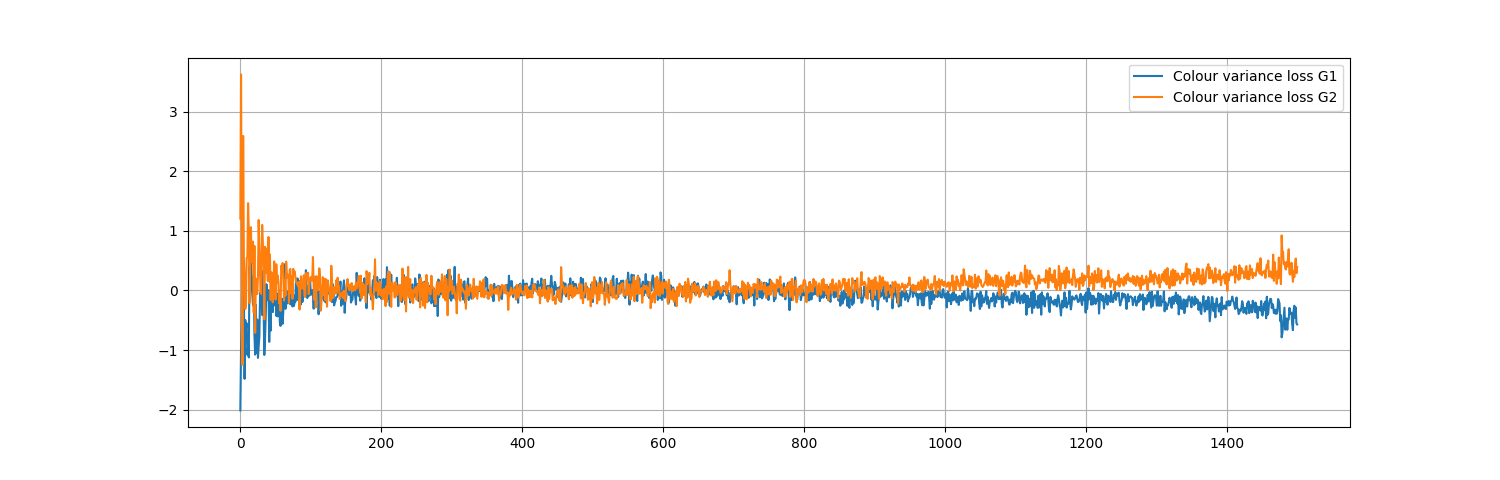
\includegraphics[width=1\textwidth]{figures/c4_unstable/train_losses/col_var/col_var_loss.png}}
    \hfill
    \subfloat[]{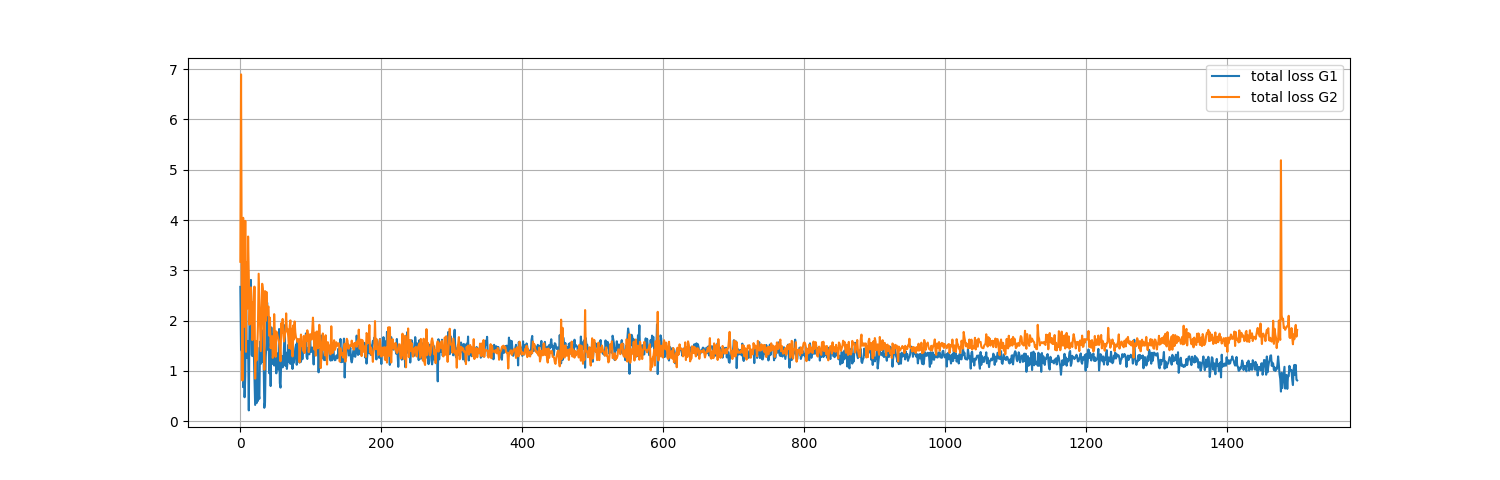
\includegraphics[width=1\textwidth]{figures/c4_unstable/train_losses/col_var/total_loss.png}}
    \caption[Loss plot for double adversarial training with colour variation loss term]{Loss plot for double adversarial training with colour variation loss term. (a) Advesarial loss terms for both respective generators. (b) Colour variation loss term for both respective generators. (c) Total loss combining both terms for both respective generators. }
    \label{fig:c3:col-var-losses}
  \end{figure}

\FloatBarrier

The visual results (Figure \ref{fig:c3:samples-col-var}) with this additional loss term show much improvement in respect to the variety across the generated data distribution, with respect to the previous experiment without the colour variance loss term (Figure \ref{fig:c3:samples-no-col-var}).
Whilst the visual results are simple in their composition, there is variety in colours generated across the generative space of both generators, which is exactly what I had been intending would happen with this additional loss term. 

In the following experiments I take these experiments further, keeping the colour diversity loss term, but replacing the adversarial loss terms with other means of measure distance and difference using common loss functions from metric learning. 
  
\section{Distance Functions}

In these further experiments I replace the adversarial loss with other means of measuring difference and distance using two common loss functions in machine learning, that come from metric learning. 
To calculate these losses efficiently the discriminator is kept in place, but here the discriminator network is used to calculate feature vector embeddings of each of the generated samples.
Pair-wise distances are calculated per-generated sample from the respective generators, where both generators are sampled using the same fixed latents during training.
The two pairwise distance loss functions used are the cosine distance and Euclidean distance, which are detailed in the following two subsections.

\subsection{Cosine Distance}

The cosine distance is between two vectors is defined as the inverse of the cosine similiarity (Eq. \ref{eq:cosine-dist}), which is used in lieue of the adversarial loss. 

\begin{equation} 
    Cosine\ distance(\vec u, \vec v) = 1 - \frac{\vec u \cdot \vec u}{|\vec u||\vec v|}
    \label{eq:cosine-dist}
\end{equation}

The mean of the cosine distance is taken for the vector embeddings from the discriminator $\vec d$ of the each respective generator $\vec d_{g_{1}}, \vec d_{g_{2}}$. 
This is calculated across the mini-batch $\vec d_{bg_{1}}, \vec d_{bg_{2}}$  and the mean is taken for the calculate the loss for the mini-batch. 
The total loss for both generators is given in Eq. \ref{eq:g1-cosine-loss} \& Eq. \ref{eq:g2-cosine-loss}.

\begin{equation} 
    G_{1}\ loss = \overline{1 - \frac{\vec d_{bg_{1}} \cdot \vec d_{bg_{2}}}{|\vec d_{bg_{1}}||\vec d_{bg_{2}}|}} + Var(B_{g_{1}}^{c}) - Var(B_{g_{2}}^{c})
    \label{eq:g1-cosine-loss}
\end{equation}

\begin{equation} 
    G_{2}\ loss = \overline{1 - \frac{\vec d_{bg_{2}} \cdot \vec d_{bg_{1}}}{|\vec d_{bg_{2}}||\vec d_{bg_{1}}|}} + Var(B_{g_{2}}^{c}) - Var(B_{g_{1}}^{c})
    \label{eq:g2-cosine-loss}
\end{equation}

The samples from training in this experiment are given in Figure \ref{fig:c3:samples-cos-cos} and the loss plots are given in \ref{fig:c3:cos-cos-losses}.

\begin{figure}[!htbp]
    \centering
    \subfloat[]{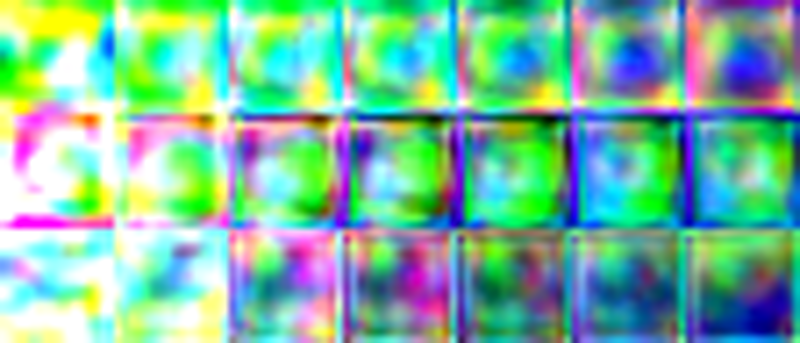
\includegraphics[width=0.45\textwidth]{figures/c4_unstable/train_samples/cos_cos/scaled_step_2_g1.png}}
    \hfill
    \subfloat[]{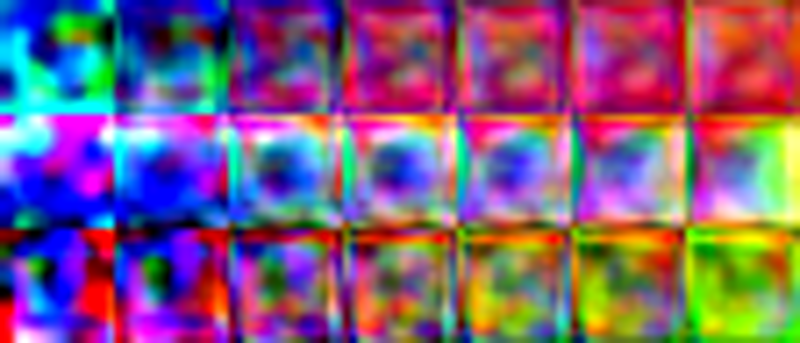
\includegraphics[width=0.45\textwidth]{figures/c4_unstable/train_samples/cos_cos/scaled_step_2_g2.png}}
    \hfill
    \subfloat[]{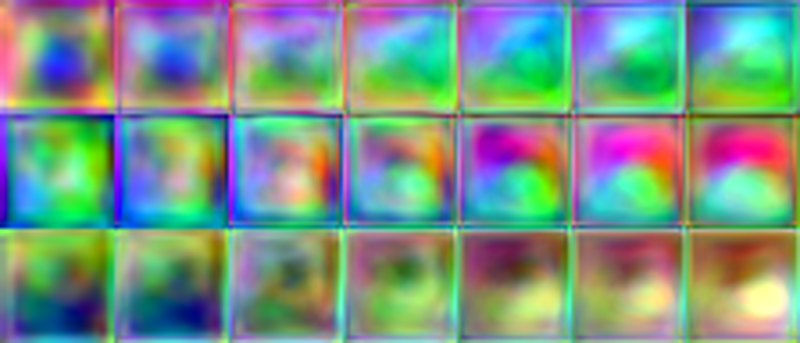
\includegraphics[width=0.45\textwidth]{figures/c4_unstable/train_samples/cos_cos/scaled_step_3_g1.png}}
    \hfill
    \subfloat[]{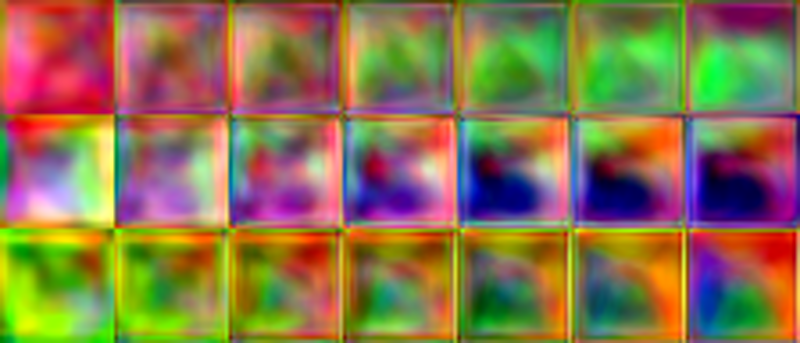
\includegraphics[width=0.45\textwidth]{figures/c4_unstable/train_samples/cos_cos/scaled_step_3_g2.png}}
    \hfill
    \subfloat[]{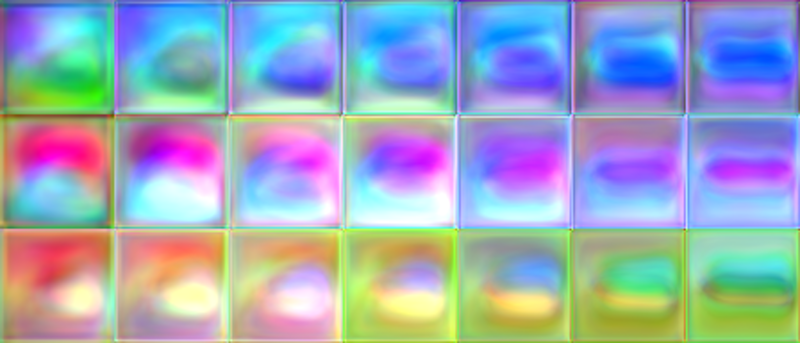
\includegraphics[width=0.45\textwidth]{figures/c4_unstable/train_samples/cos_cos/scaled_step_4_g1.png}}
    \hfill
    \subfloat[]{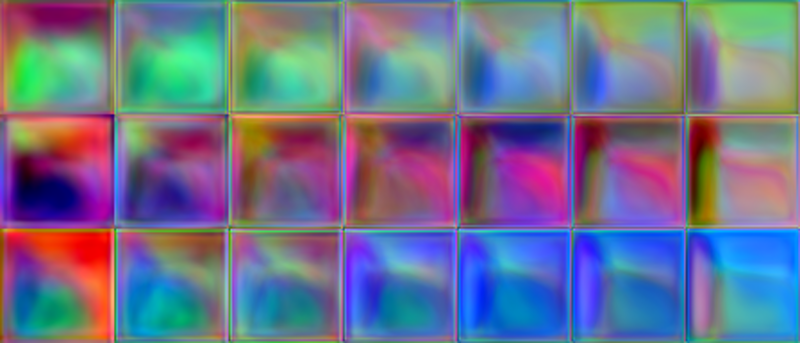
\includegraphics[width=0.45\textwidth]{figures/c4_unstable/train_samples/cos_cos/scaled_step_4_g2.png}}
    \hfill
    \subfloat[]{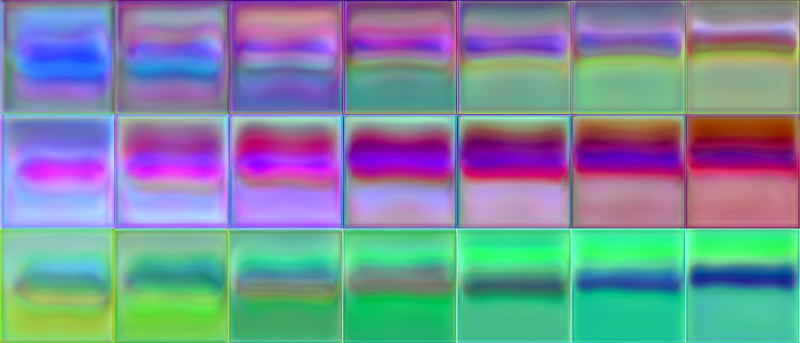
\includegraphics[width=0.45\textwidth]{figures/c4_unstable/train_samples/cos_cos/scaled_step_5_g1.png}}
    \hfill
    \subfloat[]{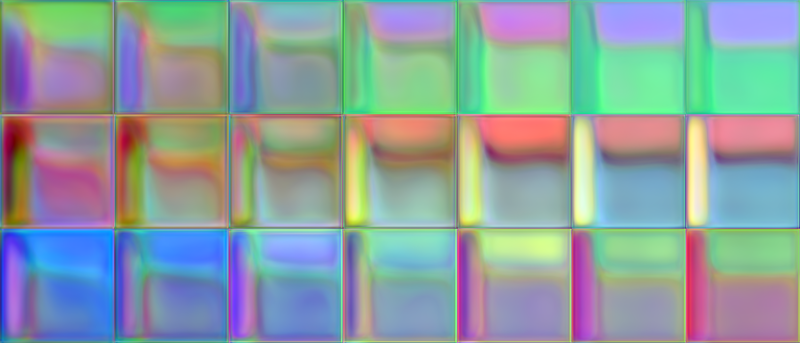
\includegraphics[width=0.45\textwidth]{figures/c4_unstable/train_samples/cos_cos/scaled_step_5_g2.png}}
    \hfill
    \subfloat[]{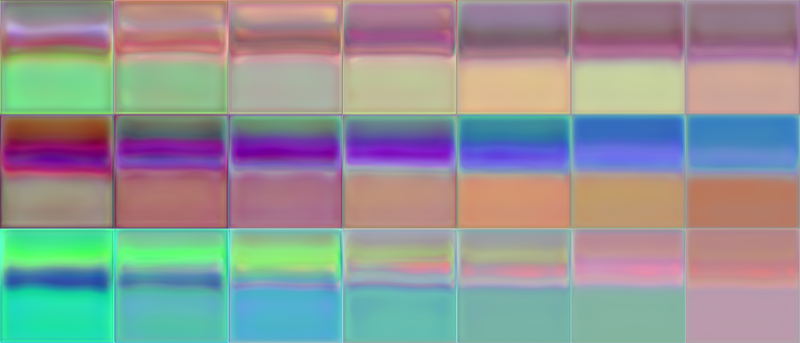
\includegraphics[width=0.45\textwidth]{figures/c4_unstable/train_samples/cos_cos/scaled_step_6_g1.png}}
    \hfill
    \subfloat[]{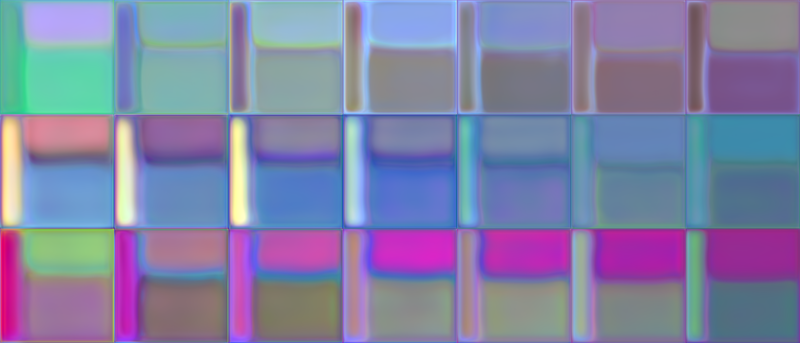
\includegraphics[width=0.45\textwidth]{figures/c4_unstable/train_samples/cos_cos/scaled_step_6_g2.png}}
    \hfill
    \caption[Training samples for two generators with cosine distance with additional colour variance loss term]{Training samples for two generators with cosine distance with additional colour variance loss term, sampled at increments of 50 iterations. The left column shows the training samples for $G_{1}$ and the right column shows the trianing samples for $G_{2}$. (a,b) Training samples at resolution 32x32 for iterations 0-300. (c,d) Training samples at resolution 64x64 for iterations 300-600. (e,f) Training samples at resolution of 128x128 for iterations 600-900. (g,h) Training samples at resolution 256x256 at iterations 900-1200. (i,j) Training samples at resolution 512x512 for iterations 1200-1500.}
    \label{fig:c3:samples-cos-cos}
  \end{figure}

  \begin{figure}[!htbp]
    \centering
    \subfloat[]{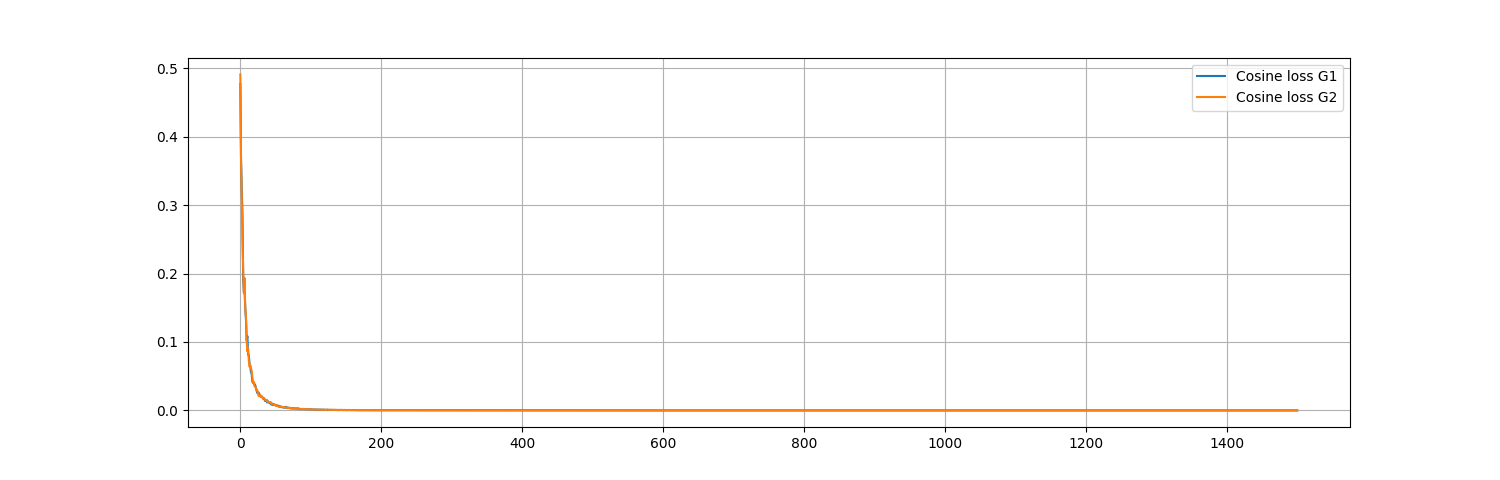
\includegraphics[width=1\textwidth]{figures/c4_unstable/train_losses/cos_cos/cosine_loss.png}}
    \hfill
    \subfloat[]{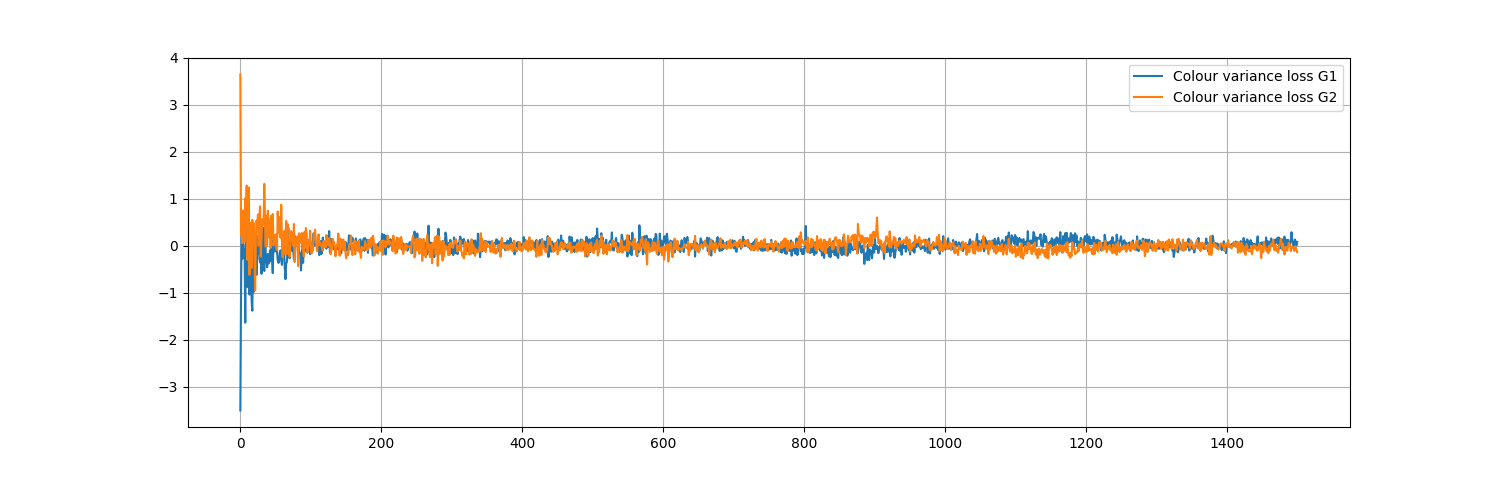
\includegraphics[width=1\textwidth]{figures/c4_unstable/train_losses/cos_cos/col_var_loss.png}}
    \hfill
    \subfloat[]{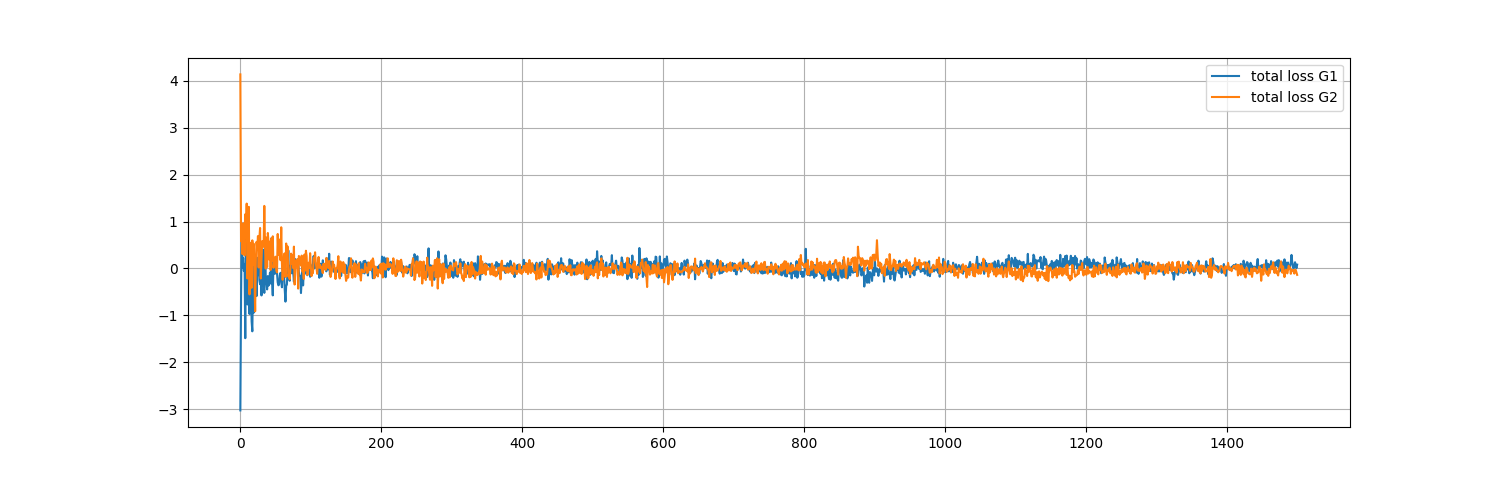
\includegraphics[width=1\textwidth]{figures/c4_unstable/train_losses/cos_cos/total_loss.png}}
    \caption[Loss plots for cosine distance training with colour variation loss term]{Loss plots for cosine distance training with colour variation loss term. (a) Cosine distance loss terms for both respective generators. (b) Colour variation loss term for both respective generators. (c) Total loss combining both terms for both respective generators. }
    \label{fig:c3:cos-cos-losses}
  \end{figure}

\subsection{Euclidean Distance}

The Euclidean distance between two vectors is shown in Eq. \ref{eq:euclid-dist}.

\begin{equation} 
    Euclidean\ distance(\vec u, \vec v) = \left \lVert \vec u - \vec v \right \rVert_2
    \label{eq:euclid-dist}
\end{equation}

The mean of the Euclidean distance is taken for the vector embeddings from the discriminator $\vec d$ of the each respective generator $\vec d_{g_{1}}, \vec d_{g_{2}}$. 
This is calculated across the mini-batch $\vec d_{bg_{1}}, \vec d_{bg_{2}}$ and the mean is taken for the calculate the loss for the mini-batch. 
The total loss for both generators is given in Eq. \ref{eq:g1-euclid-loss} \& Eq. \ref{eq:g2-euclid-loss}.

\begin{equation} 
    G_{1}\ loss = \overline{\left \lVert \vec d_{bg_{1}} - \vec d_{bg_{2}} \right \rVert_2} + Var(B_{g_{1}}^{c}) - Var(B_{g_{2}}^{c})
    \label{eq:g1-euclid-loss}
\end{equation}

\begin{equation} 
    G_{2}\ loss = \overline{\left \lVert \vec d_{bg_{2}} - \vec d_{bg_{1}} \right \rVert_2} + Var(B_{g_{2}}^{c}) - Var(B_{g_{1}}^{c})
    \label{eq:g2-euclid-loss}
\end{equation}

The samples from training in this experiment are given in Figure \ref{fig:c3:samples-euclid-euclid} and the loss plots are given in \ref{fig:c3:euclid-euclid-losses}.

  \begin{figure}[!htbp]
    \centering
    \subfloat[]{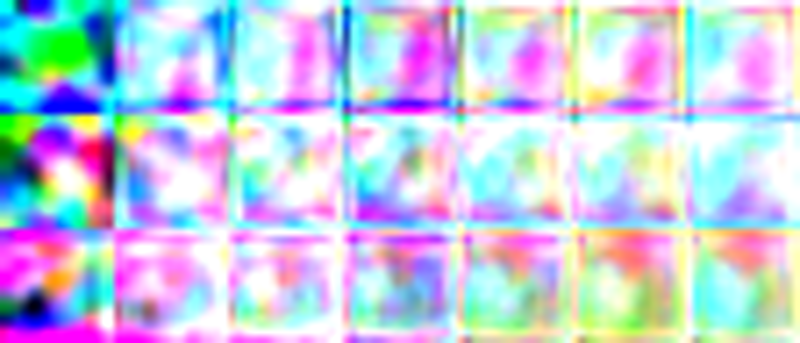
\includegraphics[width=0.45\textwidth]{figures/c4_unstable/train_samples/euclid_euclid/scaled_step_2_g1.png}}
    \hfill
    \subfloat[]{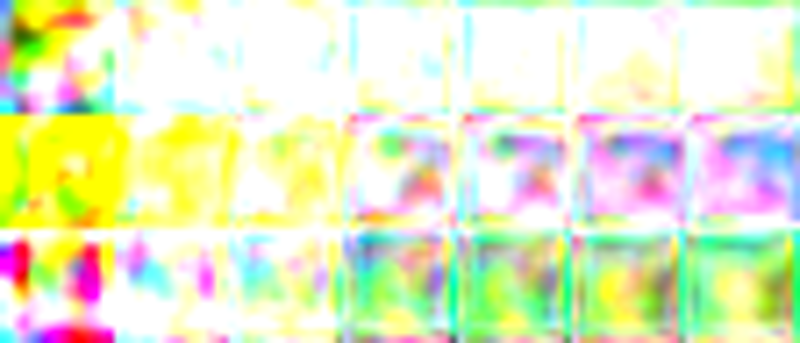
\includegraphics[width=0.45\textwidth]{figures/c4_unstable/train_samples/euclid_euclid/scaled_step_2_g2.png}}
    \hfill
    \subfloat[]{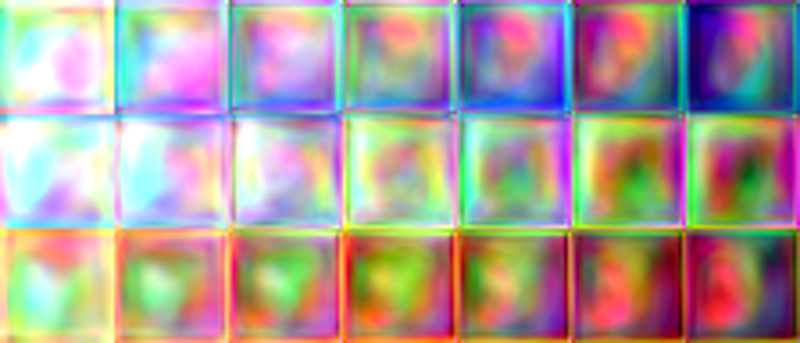
\includegraphics[width=0.45\textwidth]{figures/c4_unstable/train_samples/euclid_euclid/scaled_step_3_g1.png}}
    \hfill
    \subfloat[]{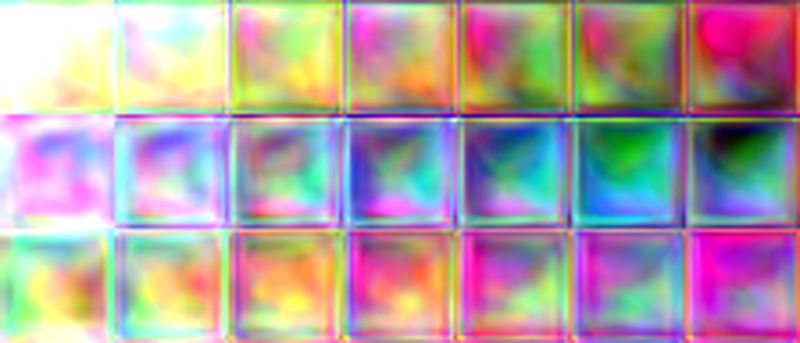
\includegraphics[width=0.45\textwidth]{figures/c4_unstable/train_samples/euclid_euclid/scaled_step_3_g2.png}}
    \hfill
    \subfloat[]{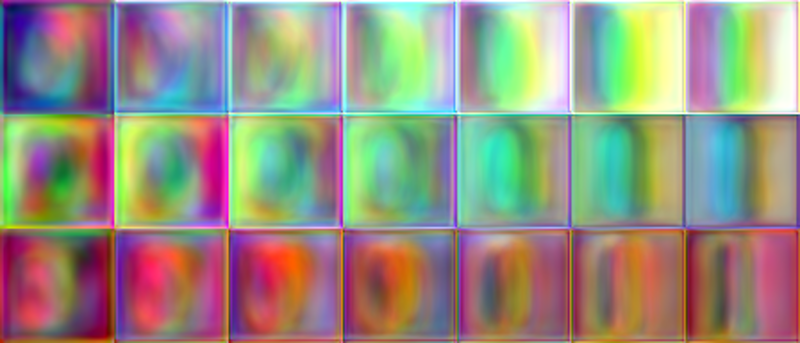
\includegraphics[width=0.45\textwidth]{figures/c4_unstable/train_samples/euclid_euclid/scaled_step_4_g1.png}}
    \hfill
    \subfloat[]{\includegraphics[width=0.45\textwidth]{figures/c4_unstable/train_samples/euclid_euclid/scaled_step_4_g2.png}}
    \hfill
    \subfloat[]{\includegraphics[width=0.45\textwidth]{figures/c4_unstable/train_samples/euclid_euclid/scaled_step_5_g1.png}}
    \hfill
    \subfloat[]{\includegraphics[width=0.45\textwidth]{figures/c4_unstable/train_samples/euclid_euclid/scaled_step_5_g2.png}}
    \hfill
    \subfloat[]{\includegraphics[width=0.45\textwidth]{figures/c4_unstable/train_samples/euclid_euclid/scaled_step_6_g1.png}}
    \hfill
    \subfloat[]{\includegraphics[width=0.45\textwidth]{figures/c4_unstable/train_samples/euclid_euclid/scaled_step_6_g2.png}}
    \hfill
    \caption[Training samples for two generators with Euclidean distance with additional colour variance loss term]{Training samples for two generators with Euclidean distance with additional colour variance loss term, sampled at increments of 50 iterations. The left column shows the training samples for $G_{1}$ and the right column shows the trianing samples for $G_{2}$. (a,b) Training samples at resolution 32x32 for iterations 0-300. (c,d) Training samples at resolution 64x64 for iterations 300-600. (e,f) Training samples at resolution of 128x128 for iterations 600-900. (g,h) Training samples at resolution 256x256 at iterations 900-1200. (i,j) Training samples at resolution 512x512 for iterations 1200-1500.}
    \label{fig:c3:samples-euclid-euclid}
  \end{figure}

  \begin{figure}[!htbp]
    \centering
    \subfloat[]{\includegraphics[width=1\textwidth]{figures/c4_unstable/train_losses/euclid_euclid/euclid_loss.png}}
    \hfill
    \subfloat[]{\includegraphics[width=1\textwidth]{figures/c4_unstable/train_losses/euclid_euclid/col_var_loss.png}}
    \hfill
    \subfloat[]{\includegraphics[width=1\textwidth]{figures/c4_unstable/train_losses/euclid_euclid/total_loss.png}}
    \caption[Loss plots for Euclidean distance training with colour variation loss term]{Loss plots for Euclidean distance training with colour variation loss term. (a) Euclidean distance loss terms for both respective generators. (b) Colour variation loss term for both respective generators. (c) Total loss combining both terms for both respective generators. }
    \label{fig:c3:euclid-euclid-losses}
  \end{figure}

  \FloatBarrier

\section{Mixing Generator Loss Functions}

In the final three experiments the adversarial, cosine distance, and Euclidean distance are mixed for training the respective generators. 

Figures \ref{fig:c3:samples-cosine-adv} \& \ref{fig:c3:cosine-adv-losses} show the training samples and loss plots for mixing the cosine distance and adversarial loss for the two respective generators. 
For this training setup $G_{1}$ is trained with Eq. \ref{eq:g1-cosine-loss} and $G_{1}$ is trained with Eq. \ref{eq:gan-g2-col-var}.

Figures \ref{fig:c3:samples-euclid-adv} \& \ref{fig:c3:euclid-adv-losses} show the training samples and loss plots for mixing the Euclidean distance and adversarial loss for the two respective generators. 
For this training setup $G_{1}$ is trained with Eq. \ref{eq:g1-euclid-loss} and $G_{1}$ is trained with Eq. \ref{eq:gan-g2-col-var}.

Figures \ref{fig:c3:samples-cosine-euclid} \& \ref{fig:c3:cosine-euclid-losses} show the training samples and loss plots for mixing the Euclidean distance and adversarial loss for the two respective generators. 
For this training setup $G_{1}$ is trained with Eq. \ref{eq:g1-cosine-loss} and $G_{1}$ is trained with Eq. \ref{eq:g2-euclid-loss}.

\begin{figure}[!htbp]
    \centering
    \subfloat[]{\includegraphics[width=0.45\textwidth]{figures/c4_unstable/train_samples/cosine_euclid/scaled_step_2_g1.png}}
    \hfill
    \subfloat[]{\includegraphics[width=0.45\textwidth]{figures/c4_unstable/train_samples/cosine_adv/scaled_step_2_g2.png}}
    \hfill
    \subfloat[]{\includegraphics[width=0.45\textwidth]{figures/c4_unstable/train_samples/cosine_adv/scaled_step_3_g1.png}}
    \hfill
    \subfloat[]{\includegraphics[width=0.45\textwidth]{figures/c4_unstable/train_samples/cosine_adv/scaled_step_3_g2.png}}
    \hfill
    \subfloat[]{\includegraphics[width=0.45\textwidth]{figures/c4_unstable/train_samples/cosine_adv/scaled_step_4_g1.png}}
    \hfill
    \subfloat[]{\includegraphics[width=0.45\textwidth]{figures/c4_unstable/train_samples/cosine_adv/scaled_step_4_g2.png}}
    \hfill
    \subfloat[]{\includegraphics[width=0.45\textwidth]{figures/c4_unstable/train_samples/cosine_adv/scaled_step_5_g1.png}}
    \hfill
    \subfloat[]{\includegraphics[width=0.45\textwidth]{figures/c4_unstable/train_samples/cosine_adv/scaled_step_5_g2.png}}
    \hfill
    \subfloat[]{\includegraphics[width=0.45\textwidth]{figures/c4_unstable/train_samples/cosine_adv/scaled_step_6_g1.png}}
    \hfill
    \subfloat[]{\includegraphics[width=0.45\textwidth]{figures/c4_unstable/train_samples/cosine_adv/scaled_step_6_g2.png}}
    \hfill
    \caption[Training samples for two generators, one with cosine distance and one with adversarial loss, both with additional colour variance loss term]{Training samples for two generators, one with cosine distance and one with adversarial loss, both with additional colour variance loss term, sampled at increments of 50 iterations. The left column shows the training samples for $G_{1}$ and the right column shows the trianing samples for $G_{2}$. (a,b) Training samples at resolution 32x32 for iterations 0-300. (c,d) Training samples at resolution 64x64 for iterations 300-600. (e,f) Training samples at resolution of 128x128 for iterations 600-900. (g,h) Training samples at resolution 256x256 at iterations 900-1200. (i,j) Training samples at resolution 512x512 for iterations 1200-1500.}
    \label{fig:c3:samples-cosine-adv}
  \end{figure}

  \begin{figure}[!htbp]
    \centering
    \subfloat[]{\includegraphics[width=1\textwidth]{figures/c4_unstable/train_losses/cosine_adv/cosine_adv_loss.png}}
    \hfill
    \subfloat[]{\includegraphics[width=1\textwidth]{figures/c4_unstable/train_losses/cosine_adv/col_var_loss.png}}
    \hfill
    \subfloat[]{\includegraphics[width=1\textwidth]{figures/c4_unstable/train_losses/cosine_adv/total_loss.png}}
    \caption[Loss plots for mixed generator losses with cosine distance and adversarial loss, both with colour variation loss term]{Loss plots for mixed generator losses with cosine distance and adversarial loss, both with colour variation loss term. (a) Losses for both respective generators, $G_{1}$ is trained with Cosine distance and $G_{2}$ is trained the adversarial loss. (b) Colour variation loss term for both respective generators. (c) Total loss combining both terms for both respective generators. }
    \label{fig:c3:cosine-adv-losses}
  \end{figure}

  \FloatBarrier

\begin{figure}[!htbp]
    \centering
    \subfloat[]{\includegraphics[width=0.45\textwidth]{figures/c4_unstable/train_samples/euclid_adv/scaled_step_2_g1.png}}
    \hfill
    \subfloat[]{\includegraphics[width=0.45\textwidth]{figures/c4_unstable/train_samples/euclid_adv/scaled_step_2_g2.png}}
    \hfill
    \subfloat[]{\includegraphics[width=0.45\textwidth]{figures/c4_unstable/train_samples/euclid_adv/scaled_step_3_g1.png}}
    \hfill
    \subfloat[]{\includegraphics[width=0.45\textwidth]{figures/c4_unstable/train_samples/euclid_adv/scaled_step_3_g2.png}}
    \hfill
    \subfloat[]{\includegraphics[width=0.45\textwidth]{figures/c4_unstable/train_samples/euclid_adv/scaled_step_4_g1.png}}
    \hfill
    \subfloat[]{\includegraphics[width=0.45\textwidth]{figures/c4_unstable/train_samples/euclid_adv/scaled_step_4_g2.png}}
    \hfill
    \subfloat[]{\includegraphics[width=0.45\textwidth]{figures/c4_unstable/train_samples/euclid_adv/scaled_step_5_g1.png}}
    \hfill
    \subfloat[]{\includegraphics[width=0.45\textwidth]{figures/c4_unstable/train_samples/euclid_adv/scaled_step_5_g2.png}}
    \hfill
    \subfloat[]{\includegraphics[width=0.45\textwidth]{figures/c4_unstable/train_samples/euclid_adv/scaled_step_6_g1.png}}
    \hfill
    \subfloat[]{\includegraphics[width=0.45\textwidth]{figures/c4_unstable/train_samples/euclid_adv/scaled_step_6_g2.png}}
    \hfill
    \caption[Training samples for two generators, one with Euclidean distance and one with adversarial loss, both with additional colour variance loss term]{Training samples for two generators, one with Euclidean distance and one with adversarial loss, both with additional colour variance loss term, sampled at increments of 50 iterations. The left column shows the training samples for $G_{1}$ and the right column shows the trianing samples for $G_{2}$. (a,b) Training samples at resolution 32x32 for iterations 0-300. (c,d) Training samples at resolution 64x64 for iterations 300-600. (e,f) Training samples at resolution of 128x128 for iterations 600-900. (g,h) Training samples at resolution 256x256 at iterations 900-1200. (i,j) Training samples at resolution 512x512 for iterations 1200-1500.}
    \label{fig:c3:samples-euclid-adv}
  \end{figure}

  \begin{figure}[!htbp]
    \centering
    \subfloat[]{\includegraphics[width=1\textwidth]{figures/c4_unstable/train_losses/euclid_adv/euclid_adv_loss.png}}
    \hfill
    \subfloat[]{\includegraphics[width=1\textwidth]{figures/c4_unstable/train_losses/euclid_adv/col_var_loss.png}}
    \hfill
    \subfloat[]{\includegraphics[width=1\textwidth]{figures/c4_unstable/train_losses/euclid_adv/total_loss.png}}
    \caption[Loss plots for mixed generator losses with cosine distance and adversarial loss, both with colour variation loss term]{Loss plots for mixed generator losses with Euclidean distance and adversarial loss, both with colour variation loss term. (a) Losses for both respective generators, $G_{1}$ is trained with Euclidean distance and $G_{2}$ is trained the adversarial loss. (b) Colour variation loss term for both respective generators. (c) Total loss combining both terms for both respective generators. }
    \label{fig:c3:euclid-adv-losses}
  \end{figure}

  \FloatBarrier

\begin{figure}[!htbp]
    \centering
    \subfloat[]{\includegraphics[width=0.45\textwidth]{figures/c4_unstable/train_samples/cosine_euclid/scaled_step_2_g1.png}}
    \hfill
    \subfloat[]{\includegraphics[width=0.45\textwidth]{figures/c4_unstable/train_samples/cosine_euclid/scaled_step_2_g2.png}}
    \hfill
    \subfloat[]{\includegraphics[width=0.45\textwidth]{figures/c4_unstable/train_samples/cosine_euclid/scaled_step_3_g1.png}}
    \hfill
    \subfloat[]{\includegraphics[width=0.45\textwidth]{figures/c4_unstable/train_samples/cosine_euclid/scaled_step_3_g2.png}}
    \hfill
    \subfloat[]{\includegraphics[width=0.45\textwidth]{figures/c4_unstable/train_samples/cosine_euclid/scaled_step_4_g1.png}}
    \hfill
    \subfloat[]{\includegraphics[width=0.45\textwidth]{figures/c4_unstable/train_samples/cosine_euclid/scaled_step_4_g2.png}}
    \hfill
    \subfloat[]{\includegraphics[width=0.45\textwidth]{figures/c4_unstable/train_samples/cosine_euclid/scaled_step_5_g1.png}}
    \hfill
    \subfloat[]{\includegraphics[width=0.45\textwidth]{figures/c4_unstable/train_samples/cosine_euclid/scaled_step_5_g2.png}}
    \hfill
    \subfloat[]{\includegraphics[width=0.45\textwidth]{figures/c4_unstable/train_samples/cosine_euclid/scaled_step_6_g1.png}}
    \hfill
    \subfloat[]{\includegraphics[width=0.45\textwidth]{figures/c4_unstable/train_samples/cosine_euclid/scaled_step_6_g2.png}}
    \hfill
    \caption[Training samples for two generators, one with cosine distance and one with Euclidean distance, both with additional colour variance loss term]{Training samples for two generators, one with cosine distance and one with Euclidean distance, both with additional colour variance loss term, sampled at increments of 50 iterations. The left column shows the training samples for $G_{1}$ and the right column shows the trianing samples for $G_{2}$. (a,b) Training samples at resolution 32x32 for iterations 0-300. (c,d) Training samples at resolution 64x64 for iterations 300-600. (e,f) Training samples at resolution of 128x128 for iterations 600-900. (g,h) Training samples at resolution 256x256 at iterations 900-1200. (i,j) Training samples at resolution 512x512 for iterations 1200-1500.}
    \label{fig:c3:samples-cosine-euclid}
  \end{figure}

  \begin{figure}[!htbp]
    \centering
    \subfloat[]{\includegraphics[width=1\textwidth]{figures/c4_unstable/train_losses/cosine_euclid/cosine_euclid_loss.png}}
    \hfill
    \subfloat[]{\includegraphics[width=1\textwidth]{figures/c4_unstable/train_losses/cosine_euclid/col_var_loss.png}}
    \hfill
    \subfloat[]{\includegraphics[width=1\textwidth]{figures/c4_unstable/train_losses/cosine_euclid/total_loss.png}}
    \caption[Loss plots for mixed generator losses with cosine distance and Euclidean distance, both with colour variation loss term]{Loss plots for mixed generator losses with cosine distance and Euclidean distance, both with colour variation loss term. (a) Losses for both respective generators, $G_{1}$ is trained with cosine distance and $G_{2}$ is trained the Euclidean distance. (b) Colour variation loss term for both respective generators. (c) Total loss combining both terms for both respective generators. }
    \label{fig:c3:cosine-euclid-losses}
  \end{figure}

\FloatBarrier

\section{Discussion}

The results for all of the training experiments using the colour variance loss term bear similiar visual and aesthetic properties. 
It is my suspicion here that it is the colour variance loss term is the component for the loss that is most instrumental in defining the direction of optimisation, and in the resulting visual results.
Whist the experiments in using distance metrics from metric learning as alternatives to the adversarial loss may have a slight impact in the differences between the visual characteristics of each result, it is clear that this impact does not make a significant impact the the overall visual aesthetic.
The difference in visual appearance could be account as much by the randomness of the inital starting parameters, or the random sequence of sampling latent variables throughout the course of training, as it is the difference in loss terms for the generator networks.
What was more important in my observations when training these models was the dynamics of the models over the course of training (albeit a very limited training run of 1500 iterations), and I settled on this arrangement because of the striking abstract visual qualities and diversity of colours across the whole generative space, which made them suitable for representing as artworks for the series of works \textit{(un)stable equilibrium}. 

Many people are surprised when I tell them that these works were made by training generative neural networks without data.
I have had many encounters where people are in disbelief that this is possible. It is commonly assumed that I must have trained these models on a dataset of abstract paintings\footnote{When presenting this work at the NeurIPS Workshop on Machine Learning for Creativity and Design, one woman was adamant that I must have use trained these networks on a dataset of painting from the Color field movement of abstract painting, and would not believe me when I told her I did not use any training data.}, or a synthetic dataset of colour gradients. 
The resemblance here to paintings by Mark Rothko are not lost on me in these experiments, and indeed that was the first thing that sprung to mind when I performed the first training run with the colour variance loss term.\footnote{I even labelled the folder `rothko-esque' on my computer after performing the inital training run with the colour variance loss term.} 
This however, seems to be a happy accident, or at least, my aesthetic preferences were the `meta-heuristic' guiding me in my development of the code of the course of several weeks that finally led to creating a training ensemble of networks that created works that share this uncanny resemblance.

The time taken to train these models is incredibly short (with respect to the time taken for training standard generative models such as GANs). 
1500 iterations is the length of training used in all these experiments, and the visual formation begins to the stabilise after 1000 iterations. 
This could be due to a convergence towards some kind of stable equilibrium, but could also be in part determined by the progressive growing training arangement in the StyleGAN models, as by the time the models are scaled up to the resolution 256x256, the overall shape of the generations starts to stabilise, and this could be related to the number of parameters being trained and the diminishing gradients that reach the lower-layers of the network, where structural formation of the images takes place.
My experiments in Chapter \ref{ch:net_bend} go into more detail exploring the functions of different layers within the generators of GANs. 


\section{Conclusion}

The work in this chapter was significant for a number of reasons, the artistic value and its impact in the artwork has already been mentioned. 
From the perspective of the narrative of this thesis though it was important for other reasons. 
This was the first breakthrough in the aim of developing a data-divergent, or more appropriately a data-agnostic way of training generative neural networks, such that they create something completely novel. 
The way this was achieved by leaning on my significant experience of coding and training machine learning system, which I had grown to be quite comfortable with; to the degree that I could playfully experiment with the code and build neural networks ensembles where gradient based learning was able to be performed successfully.
The impact that this work has had has been more signifcant in the reception of the series of artworks \textit{(un)stable equilibrium} from my first experiments with this way of training generative neural networks (Figure \ref{fig:c3:original-experiments}), this artistic reception is detailed in \S \label{c7:sec:unstable_eq}.

A number of orthodoxies of machine learning are deliberately challenged in this work. 
The first, that data is needed to ‘learn’ or happen upon culturally relevant representations. That optimisation must be convex, that the goal of optimization must be clearly defined in a formula derived from a theory taken from statistics, physics or some branch of mathematics. 
That regularisation of training comes from the stochastic nature of data, and not from the dynamics of the models themselves. 

The following chapter builds on this work, though instead of focusing on training models from scratch, I took my next experiments into fine-tuning models that had already been trained.